% VLDB-Template enhances the ACM master template, acmart.cls v2.19 (2026/06/27):
% https://www.acm.org/publications/proceedings-template
% The ACM Latex guide provides further information about the ACM template
%
% This bundle pins acmart.cls v2.19 (rather than relying on whatever version
% ships with an author's local TeX install or Overleaf project) to guarantee
% consistent formatting across all PVLDB submissions.

\documentclass[sigconf, nonacm]{acmart}

%%% do not modify the following VLDB block %%
%%% VLDB block start %%%
\usepackage{pvldb}% VLDB/PVLDB formatting overrides, see pvldb.sty for details.
                      % Do not remove -- required for consistent proceedings
                      % formatting across all VLDB submissions.
%%% VLDB block end %%%

\usepackage{multirow}
\usepackage{graphicx}
\usepackage{array}
\let\Bbbk\relax
\usepackage{amssymb}
\usepackage{tabularx}

%% The following must be set for each paper (values below are placeholders).
%% Everything else (volume/issue/year defaults, the PVLDB Reference Format
%% block, license footer, and Artifact Availability block) is handled by
%% pvldb.sty -- see that file if you need to change shared defaults.
\renewcommand\vldbdoi{XX.XX/XXX.XX}
\renewcommand\vldbpages{XXX-XXX}
% leave empty if no availability url should be set
\renewcommand\vldbavailabilityurl{https://github.com/SJieNg123/sqlite-research} 

\begin{document}
\title{Preprocessing Cost Accounting for SQLite Cold-Start Prefetch in Serverless and Edge Deployments: Why Faster First Queries Don't Mean Faster Cold Starts}

%%
%% The "author" command and its associated commands are used to define the authors and their affiliations.
\author{Shi Jie Ng}
\affiliation{%
  \institution{National Tsing Hua University}
  \city{Hsinchu}
  \country{Taiwan}
}
\email{shijieng@gapp.nthu.edu.tw}

\author{Yun-Chih Chen}
\affiliation{%
  \institution{National Tsing Hua University}
  \city{Hsinchu}
  \country{Taiwan}
}
\email{yunchih@cs.nthu.edu.tw}

%%
%% The abstract is a short summary of the work to be presented in the
%% article.

\begin{abstract}
Serverless functions backed by SQLite face a persistent cold-start bottleneck: after an idle period the OS page cache is evicted, and the first query runs two to three orders of magnitude slower than subsequent ones. Prefetching is the natural remedy, and existing work evaluates it by post-prefetch first-query latency. We show that this metric can misrank strategies, because in a serverless request the prefetch itself sits on the user-visible critical path. We introduce a critical-path cost accounting that decomposes cold-start latency into a cold file open, per-page delivery, and the first query, and evaluates it under two deployment boundaries: an integrated warm-process model that reuses an open handle, and an external warmer that pays the cold open. The framework uses only standard POSIX interfaces and requires no modification to SQLite, the kernel, or the runtime. Under this accounting the ranking reverses. A full working-set cache dump minimizes first-query latency (80\% to 91\% reduction) yet regresses end-to-end cold starts by roughly an order of magnitude on broad workloads, because its 0.8 to 7 ms delivery cost dominates the response. The robust operating point is frugal coverage: a set under 2 MB that covers the B+tree interior navigation path yields a 25\% to 30\% end-to-end reduction across skewed and uniform read workloads, and hot-leaf prefetching helps only under an independently verified hotspot. At matched footprint, a frequency-ranked dump is statistically indistinguishable from a type-aware selector, so footprint and coverage carry the result rather than selector sophistication. The design rule holds under write churn, memory pressure, 10× database scaling, and a moving hotspot, and the first-query effectiveness of the selected page sets carries over to a separate-host Apache OpenWhisk deployment.
\end{abstract}

\maketitle

%%% do not modify the following VLDB block %%
%%% VLDB block start %%%
\vldbtopmatter
%%% VLDB block end %%%

\section{Introduction}\label{sec:introduction}

\subsection{Background}\label{sec:background}

\subsubsection{Serverless SQLite as a Growing Deployment Target}\label{sec:serverless-sqlite}

Serverless computing has become a dominant execution model for cloud applications, offering transparent scaling, fine-grained billing, and simplified operations. A growing share of serverless workloads is stateful and accesses persistent data in embedded databases co-located with function instances. SQLite is the most widely deployed engine for this role: Gaffney et al. \cite{Gaffney2022} estimate that over one trillion SQLite databases are in active use and identify edge computing as a key emerging use case for its zero-configuration data management. FaaS platforms such as AWS Lambda, Azure Functions, and Google Cloud Functions let functions mount persistent storage or use ephemeral local disk, making SQLite a natural choice for function-local state, configuration, and lightweight analytics. In such deployments SQLite is the storage layer of the function, and its latency contributes directly to the function's response time. Production edge databases and object-storage-backed SQLite systems ~\cite{CloudflareD1, SqliteWebVfs, Turbolite} place the same local storage layer on the request path.

\subsubsection{Warm Container, Cold Data}\label{sec:warm-container}

Wang et al. \cite{Wang2018} measured over 50,000 function instances across AWS Lambda, Azure Functions, and Google Cloud Functions and showed that platforms reuse containers or virtual machines across invocations, so a warm runtime is the common case. They also observed frequent resource contention between co-located functions. Such contention is consistent with the OS reclaiming file-backed pages between invocations, so pages cached by one invocation may no longer be resident when the next arrives. Shahrad et al. \cite{Shahrad2020} characterized production traces from Azure Functions and found that invocation frequencies span eight orders of magnitude and that inter-invocation intervals are highly variable, which makes future invocations hard to predict. Platforms therefore combine keep-alive and prewarming policies that hold the runtime warm while allowing memory to be reclaimed during idle periods. The result is the state this paper targets: the function runtime and its SQLite handle are alive, but the OS page cache backing the database file has been evicted. We refer to this state as warm container, cold data, and use the hyphenated form warm-container, cold-data as a modifier throughout.

\subsection{Motivation}\label{sec:motivation}

Container-level cold-start optimization has advanced rapidly. The histogram-based prewarming policy of Shahrad et al. \cite{Shahrad2020} raises the fraction of invocations that land on a warm container, and Catalyzer \cite{Du2020} reaches sub-millisecond function startup through checkpoint/restore and the sfork primitive. Neither technique restores the OS page cache: a checkpoint does not carry file-backed pages, and prewarming keeps the runtime alive while memory is reclaimed. As these techniques succeed, the cold-start penalty that remains sits in the data path.

That penalty is not small. On our reference database (Section~\ref{sec:refdb}), the first query after a cold OS page cache takes 500 to 1067 µs depending on the workload, against 1 to 3 µs once the cache is warm (Section~\ref{sec:workloads}), a slowdown of two to three orders of magnitude. The storage-layer penalty is therefore in the same sub-millisecond regime as container startup itself, so even an optimally warmed container leaves the data path as the dominant remaining cost.

The cost arises from a dependent fault chain. Each query walks the B+tree from root to leaf, and each missing page must be fetched before the next page address is known. On local NVMe each link costs microseconds. When SQLite is served from object storage over HTTP range requests ~\cite{SqliteWebVfs, Turbolite}, each link becomes a multi-millisecond GET and the same chain is amplified by orders of magnitude. This paper quantifies the chain at the local-storage tier and leaves the remote tier to future work (Section~\ref{sec:conclusion}).

\subsection{Challenges and Problem Statement}\label{sec:challenges}

Prefetching the pages that the first query will touch is the natural remedy for the warm-container, cold-data state. Three challenges stand in the way, and no prior approach addresses all of them at once.

\textbf{Challenge 1: Targeting.} The OS page cache operates on file blocks and has no view of SQLite's B+tree. Kernel readahead detects sequential access and misses the non-sequential root-to-leaf traversal that every query performs, whereas loading an entire working set spends I/O on pages the first query never touches. The prefetch set must be small enough to be cheap and sound enough to cover the navigation path of any first query. How to select such a set, and whether structural page-type knowledge or observed access frequency selects it better, is an open question.

\textbf{Challenge 2: Cost Accounting.} Prefetching is not free. Prior work optimizes the post-prefetch first-query latency and implicitly assumes that a lower first query yields a faster cold start. In a serverless request the user blocks on the function's response, so the time spent opening the file and issuing per-page prefetch operations extends the response directly. When this preprocessing cost exceeds the first-query reduction, prefetching slows the cold start.

\textbf{Challenge 3: Deployability.} Functions run in restricted runtimes where modifying the OS kernel, the storage firmware, or the database engine is usually infeasible. Solutions that patch SQLite \cite{VanDeBogart2009}, move transaction logic into the FTL \cite{Kang2013}, or add kernel modules \cite{Leis2023} cannot be deployed there. A practical mechanism must operate at the application layer through standard OS interfaces without privileged access.

The three challenges are coupled. A well-targeted set that ignores its own cost can be net-harmful, a cost-aware but poorly targeted set brings no benefit, and either one is moot if it cannot be deployed. This paper addresses all three together.

\subsection{Our Contributions}\label{sec:contribution}

This paper presents a non-intrusive prefetch framework for SQLite cold starts in serverless and edge deployments and, with it, a methodology for evaluating such prefetch on the user-visible critical path. Our contributions are:

\textbf{Critical-path cost accounting (Section~\ref{sec:methodology})}. We decompose cold-start latency into a cold file open, per-page delivery, and the first query, and evaluate it under two deployment boundaries: a warm-process model that reuses an open SQLite handle, and an external-warmer model that pays the cold open. We further separate page selection from page delivery so that selection accuracy is not conflated with delivery residency. To our knowledge, this is the first evaluation of SQLite cold-start prefetch that charges the prefetch itself to the critical path, and it exposes a systematic gap between first-query and end-to-end rankings.

\textbf{A frugal-coverage design rule (Sections~\ref{sec:strategy} and~\ref{sec:evaluation})}.  Charging preprocessing reverses the naive ranking. The full working-set cache dump minimizes first-query latency but regresses end-to-end cold starts by roughly an order of magnitude on broad workloads, because delivery cost dominates. The robust operating point is a set under 2 MB that covers the B+tree interior navigation path, which yields a 25\% to 30\% warm-process end-to-end reduction across skewed and uniform read workloads. Hot-leaf prefetching is a conditional add-on that helps only under an independently verified hotspot, and at matched footprint a frequency-ranked dump is statistically indistinguishable from the type-aware selector. Page-type knowledge therefore serves as an interpretable coverage guarantee that stays stable when the read hotspot moves, rather than as a uniquely faster selector. A physical layout rewriter that clusters interior pages at the file head is a negative result under our workloads.

\textbf{A deployable toolchain and its validation (Sections~\ref{sec:deployment},~\ref{sec:eval-robustness}, and \ref{sec:eval-portability}).} The framework uses only standard POSIX interfaces (mmap, mincore, madvise) and modifies neither SQLite, the kernel, the storage firmware, nor the serverless runtime. We validate the design rule across six robustness axes on a controlled workstation: write churn, memory pressure, multi-process cache sharing, workload instantiation, database scaling, and a moving read hotspot. We then deploy the same toolchain on a separate-host Apache OpenWhisk runtime, where every strategy that is strongly effective on the workstation remains effective and per-cell first-query effectiveness ranks correlate at Spearman $\rho$ of 0.76 to 0.81.

\textbf{Scope of evidence.} The workstation is the sole basis for the end-to-end cost accounting and the design rule. There we measure the first-query, delivery, and cold-open terms directly and instantiate the two deployment boundaries as models of serverless keep-alive behavior rather than as traces from a commercial platform. The OpenWhisk deployment measures deployability and relative first-query effectiveness only, so it establishes neither cross-platform end-to-end ranking nor absolute-latency or hardware portability. We do not measure commercial FaaS providers, other hardware classes, or the remote object-storage tier, for which we claim only that the same dependent fault chain motivates analogous accounting. Section~\ref{sec:discussion} discusses these limitations further.

Section~\ref{sec:related} surveys related work. Section~\ref{sec:fundamentals} reviews SQLite's B+tree layout and defines the warm-container, cold-data measurement model. Section~\ref{sec:methodology} presents the cost model, the selection–delivery decomposition, and the measurement and statistical protocol. Section~\ref{sec:strategy} describes the prefetch strategies and physical layouts. Section~\ref{sec:setup} describes the platform, reference database, and workloads. Section~\ref{sec:evaluation} reports results, Section~\ref{sec:discussion} discusses limitations, and Section~\ref{sec:conclusion} concludes.

\section{Related Work}\label{sec:related}

Table~\ref{tab:capability} positions this work against prior art along three axes: structural targeting of B+tree pages, cost accounting of the prefetch on the critical path, and non-intrusive deployment. No surveyed system provides all three, and the cost-accounting column is empty throughout.

\subsection{OS-Level and Application-Directed Prefetching}\label{sec:os-prefetch}

OS prefetching begins with Smith~\cite{Smith1978}, whose one-block lookahead exploits sequential access and includes a cost model for when to prefetch. Anticipatory scheduling~\cite{Iyer2001} addresses deceptive idleness by waiting briefly for the next nearby request. Both trade time for locality because the OS lacks application semantics, and both assume seek-dominated disks, a premise that does not hold on NVMe. Our cold start also has no access history for the first query, so we deduce the required pages from the B+tree structure instead of predicting them. libprefetch ~\cite{VanDeBogart2009} closes the semantic gap by letting the application declare future reads so the OS can issue them in C-LOOK order, accelerating SQLite table scans by up to 20× on HDDs. Its gains come from seek avoidance with reorder buffers of hundreds of megabytes, and its SQLite integration modifies roughly 500 lines of engine source. In our regime the bottleneck is per-page cache-miss and syscall cost rather than seek time, so every prefetched page extends the critical path and frugality replaces volume. Section~\ref{sec:eval-attribution} reproduces libprefetch's ordering effect as a delivery-order arm and finds its NVMe residue confined to the synchronous delivery term.

\subsection{Buffer-Pool Warming and Learned Prefetching}\label{sec:buffer-warming}

Buffer management was formalized by Effelsberg and Härder~\cite{Effelsberg1984}. Learned prefetchers build on it: Chen et al.~\cite{Chen2021} cast page prediction as classification and report 76\% to 87\% precision and recall, but evaluate prediction accuracy rather than end-to-end latency, quantify neither inference overhead nor mis-prefetch cost, and train on warm-start traces that a cold cache does not provide. Pre-Buffer~\cite{Yi2026} targets hit-rate collapse when hotspots shift by predicting the next cycle's hot set from per-cycle records, loaded by a background thread. It faults Chen et al. for ignoring prefetch overhead, yet measures only hit-rate recovery and total execution time, and its background thread keeps that overhead off the user-facing path. In a serverless cold start the prefetch runs on the critical path before the first query, which is what makes syscall-level cost accounting necessary. Leaper~\cite{Yang2020}, a learned LSM prefetcher, depends on access skew, consistent with our finding that hotspot-based selection helps only when a hotspot exists. Funke et al.~\cite{Funke2022} show in query compilation that preprocessing latency can dominate short-query response and that a lightweight mechanism beats a heavy one below a break-even point, the same critical-path lesson we draw in the I/O domain. Section~\ref{sec:eval-attribution} ports the selection cores of the InnoDB buffer-pool dump and of Pre-Buffer as competitive baselines and evaluates a learned transition model in the lineage of Chen et al. under the same accounting.

\subsection{SQLite Storage: mmap and the Write Path}\label{sec:write-path}

Crotty et al.~\cite{Crotty2022} argue against \texttt{mmap} as a buffer-pool replacement but exempt read-only workloads whose working set fits in memory. Our use sits in that exception and is narrower still: SQLite's pager retains caching and recovery, and we use ~\texttt{mmap}, ~\texttt{mincore}, and \texttt{madvise} only as a prefetch-hint channel. vmcache~\cite{Leis2023} retains DBMS-controlled eviction through \texttt{madvise} but finds that Linux page-table primitives do not scale at high frequency and adds a kernel module. We occupy the opposite corner, about 92 \texttt{madvise} calls per cold start, unprivileged and application-layer, where standard interfaces suffice. A separate strand optimizes SQLite's write path in mobile and embedded settings through engine, journaling, or flash translation layer (FTL) changes~\cite{Jeong2013, Kang2013, Kim2012, Oh2015}. All require invasive modification and target write amplification, which is orthogonal to read cold start. Gaffney et al.~\cite{Gaffney2022}, the most comprehensive SQLite evaluation, prewarm every table before measurement and thus treat cold start as noise to remove rather than a cost to measure.

\subsection{Serverless Cold Start and SQLite at the Edge}\label{sec:serverless-coldstart}

Serverless cold start is characterized at the platform level by container reuse~\cite{Wang2018} and unpredictable invocation intervals~\cite{Shahrad2020}, which together produce the warm-container, cold-data state of Section~\ref{sec:warm-container}. Catalyzer~\cite{Du2020} reaches sub-millisecond startup through checkpoint/restore, but it does not restore the OS page cache. At the storage layer, SQLite increasingly runs from edge and object-storage backends~\cite{CloudflareD1,SqliteWebVfs,Litestream,SqlJsHttpvfs,Turbolite}, where a custom VFS turns each page I/O into an HTTP range request and cold start becomes the headline metric~\cite{Turbolite}. Closest to our selection lever is the .dbi helper of sqlite\_web\_vfs ~\cite{SqliteWebVfs}, which gathers navigation-critical interior and metadata pages into a sidecar that the VFS prefetches, validating interior-first selection in production. It is a sidecar for a read-only HTTP VFS, publishes no accounting of the prefetch cost, and stops at page types. We operate on the local OS page cache, add no file, support read-write workloads, charge the prefetch to the critical path, and additionally evaluate an access-frequency leaf lever. Section~\ref{sec:eval-attribution} returns to .dbi's copy-rather-than-reorder design when discussing our layout rewriter.

\begin{table}[htbp]
\centering
\small
\setlength{\tabcolsep}{5pt}
\caption{
Positioning against prior art ($\checkmark$ full, $\checkmark$* partial, $\times$ absent). Structural targeting: B+tree page-type or access-frequency awareness. Cost accounting: open and deliver preprocessing charged to the end-to-end critical path. Non-intrusive: no SQLite, kernel, or FTL source modification.}
\begin{tabular}{@{}l ccc@{}}
\toprule
\textbf{Approach} & \shortstack{\textbf{Structural}\\\textbf{targeting}} & \shortstack{\textbf{Cost}\\\textbf{accounting}} & \shortstack{\textbf{Non-intrusive}\\\textbf{deployment}} \\
\midrule
OS readahead~\cite{Smith1978,Iyer2001} & $\times$ & $\times$ & $\checkmark$ \\
libprefetch~\cite{VanDeBogart2009} & $\checkmark$ & $\times$ & $\times$ \\
Learned prefetch~\cite{Chen2021,Yi2026} & $\checkmark$* & $\times$ & $\times$ \\
\texttt{.dbi} web VFS~\cite{SqliteWebVfs} & $\checkmark$* & $\times$ & $\checkmark$ \\
\midrule
\textbf{Our work} & $\checkmark$ & $\checkmark$ & $\checkmark$ \\
\bottomrule
\end{tabular}
\label{tab:capability}
\end{table}

\section{SQLite Cold-Start Fundamentals}\label{sec:fundamentals}

\subsection{B+tree Storage and Page Types}\label{sec:btree}

SQLite stores a database in a single file of fixed-size pages, 4 KB in our configuration, and each table and index is a B+tree over those pages~\cite{Gaffney2022}. Interior pages hold keys and child pointers, and leaf pages hold row data or index entries. Page 1 holds the file header and the root of the \texttt{sqlite\_master} schema tree, and the root page of each user table or index is recorded in the \texttt{rootpage} column of \texttt{sqlite\_master} and is usually a low page number. Our reference database of 600,000 rows (Section~\ref{sec:refdb}) occupies about 103 MiB and contains 92 interior pages, 51 in the table B+tree and 41 in the secondary index, totaling 368 KB, plus 26,239 leaf pages.

Standard B+tree fanout makes interior pages 0.35\% of the file, yet every query traverses them from root to leaf. A single point query touches only the pages on one root-to-leaf path, typically three to four including the leaf, whereas a workload's accumulated interior set converges to all 92. This distinction separates two prefetch targets: a per-query path of a few pages and a workload-wide interior skeleton of 368 KB. Both are small, and both lie on the navigation path that no query can skip. This arithmetic is a direct consequence of B+tree fanout rather than a property specific to SQLite, and it is what makes a frugal prefetch set possible.

\subsection{Cold-Start Mechanics}\label{sec:coldstart-mechanics}

With an empty OS page cache, the first query must fetch every page on its root-to-leaf path from disk, one dependent fault at a time, because each child pointer is unknown until its parent page is resident. On commodity NVMe each fault costs 5 to 100 µs, and the chain sums to the cold first-query latencies of 500 to 1067 µs reported in Section~\ref{sec:workloads}, two to three orders of magnitude above the warm case. The interior pages on that chain are few and known in advance (Section~\ref{sec:btree}), so a prefetch that makes them resident before the first query removes the interior faults. Whether this improves the end-to-end cold start depends on which pages are selected (Section~\ref{sec:strategy}) and on what the prefetch itself costs (Section~\ref{sec:methodology}).

\subsection{The Warm-Container, Cold-Data Measurement Model}\label{sec:measurement-model}

Our measurement model instantiates the warm-container, cold-data state of Section~\ref{sec:warm-container}. Before each measurement we keep the process-layer state warm, namely the SQLite handle, prepared statements, and the mmap mapping, and clear every software cache below the process layer. Table~\ref{tab:measurement-model} lists the state of each layer at measurement time and the serverless condition it models.

This design is deliberate on three counts. It matches deployments that reuse containers, where the runtime and handle survive and only the page cache must be re-established. It isolates the variable under study, since SQLite parser and optimizer startup is a constant that no prefetch strategy changes. And it reduces variance, because a fresh process per measurement adds 50 to 200 \textmu s of initialization noise that would require more repetitions to suppress. The one bias the model introduces is a warm CPU cache and TLB, which we estimate at 1 to 3 \textmu s, below 1\% of the cold baseline. Section~\ref{sec:protocol} gives the operational protocol, including cache clearing, residency verification, and cell rejection.

\begin{table}[htbp]
\centering
\caption{State of each layer at measurement time and the serverless wake-up condition it models.}
\label{tab:measurement-model}
\begin{tabular}{p{0.15\linewidth}p{0.36\linewidth}p{0.36\linewidth}}
\toprule
\textbf{Layer} & \textbf{State at measurement} & \textbf{Serverless condition modeled} \\
\midrule
OS page cache & Emptied via system-wide cache drop, verified $<1\%$ resident via \texttt{mincore} & Reclaimed during idle period or memory contention \\
Disk I/O & Pages must be read from disk (\texttt{majflt} $>0$) & Physical I/O required on cold fault \\
SQLite handle and pager & Pre-opened, statements prepared & Function runtime reused, handle preserved \\
\texttt{mmap} region & Mapping established, pages not faulted & Virtual memory mapping intact, pages absent \\
CPU caches / TLB & Warm (harness code has run) & Processor state preserved across wake-up \\
\bottomrule
\end{tabular}
\end{table}

\section{Cold-Start Cost Model and Measurement Methodology}\label{sec:methodology}

\subsection{The End-to-End Cost Model}\label{sec:cost-model}

The first-query latency $t_{\text{fq}}$ measures only the SQL query's wall-clock time and excludes the cost of issuing the prefetch. From the user's perspective the relevant quantity is the time from function wake-up to query completion, and in a serverless request every microsecond of prefetch preprocessing lands on that path. We decompose the preprocessing into two syscall-level terms. The cold-open cost $t_{\text{open}}$ is the cost of opening the database file with a cold cache. It is constant for a given layout and independent of the prefetch strategy, about 179 \textmu s on our platform (Section~\ref{sec:eval-tradeoff}). The delivery cost $t_{\text{deliver}}$ is the cost of issuing the prefetch operations, whether asynchronous madvise hints or synchronous pread calls, and scales linearly with the number of pages in the prefetch set. The warmer reports both terms separately.

Two deployment models follow, differing only in whether $t_{\text{open}}$ is paid:

\begin{equation}\label{eq:e2e_ext}
    \text{e2e}_{\text{ext}} = t_{\text{open}} + t_{\text{deliver}} + t_{\text{fq}}
\end{equation}

\begin{equation}\label{eq:e2e_warm}
    \text{e2e}_{\text{warm}} = t_{\text{deliver}} + t_{\text{fq}}
\end{equation}

The external-warmer model (Eq.~\ref{eq:e2e_ext}) corresponds to a separate process, such as a sidecar, that prefetches on every invocation and must open the database file itself. It is the pessimistic bound. The warm-process model (Eq.~\ref{eq:e2e_warm}) corresponds to the warm-container, cold-data state of Section~\ref{sec:warm-container}: the application is running, its SQLite handle is open, and the prefetch reuses that handle. This is the model we advocate for serverless keep-alive and edge-worker deployments. The baseline in both models is$t_{\text{fq}}$ with no prefetch, measured through the handle opened before cache clearing, so it contains no open cost and is identical across models.

The prefetch set itself is computed offline by a separate pipeline (a cold clear, a workload warmup, and a mincore snapshot) and reused across many cold starts. Its cost is amortized and does not enter the per-event critical path. Section~\ref{sec:eval-robustness} shows that under a stationary read hotspot the set does not decay across 50,000 write mutations, whereas a moving hotspot does require refreshing a frequency-based plan.

The trade-off follows directly: prefetch helps when $t_{\text{deliver}}$ is small relative to the first-query reduction and hurts when $t_{\text{deliver}}$ dominates. Section~\ref{sec:eval-tradeoff} quantifies both cases.

\subsection{Selection--Delivery Decomposition}\label{sec:selection-delivery}

The \texttt{madvise(MADV\_WILLNEED)} hint is asynchronous. The kernel records the hint, starts background readahead, and returns, so whether a page is resident when the first query runs depends on scheduling and I/O completion. The first-query latency under asynchronous hints therefore conflates two factors: whether the selected set is the right one (\textit{selection}) and how much of it is resident in time (\textit{delivery}). We separate them by running every prefetch set under the two delivery modes. Synchronous pread returns only after all pages are resident and gives $t_{\text{fq,pread}}$, the lower bound a perfectly delivered set can reach. Asynchronous hints give $t_{\text{fq}}$,async together with the delivery rate observed via mincore. Their gap is the delivery loss:

\begin{equation}\label{eq:delivery_loss}
    \text{delivery\_loss} = t_{\text{fq,async}} - t_{\text{fq,pread}}
\end{equation}

Mechanisms between the two can move delivery toward the bound, and one of them is cheap
enough that we adopt it as a third mode rather than defer it. Because the kernel honours a
range hint only up to its readahead window, issuing one hint per window-sized chunk turns a
single large request into a sequence the kernel satisfies in full. We call this
\textit{window-chunked} asynchronous delivery, and Section~\ref{sec:eval-attribution}
reports every strategy under it alongside the per-page mode. Mechanisms that need a
different submission interface, such as \texttt{io\_uring}, or a different point in the
function lifecycle remain outside our scope.

Two details of the asynchronous path affect the measurements. First, the kernel readahead
window bounds what one range hint can deliver. With \texttt{read\_ahead\_kb} = 128 on our
platform the window is $W = 32$ pages, and one
\texttt{posix\_fadvise(POSIX\_FADV\_WILLNEED)} over a range of $n$ pages delivers
$\min(n, W)$ pages from the head of that range while returning success either way.
\texttt{POSIX\_FADV\_SEQUENTIAL} doubles $W$ to 64. This is why we observe only 32 of 92
requested interior pages delivered from one range hint on the default layout. All per-page
strategies in Section~\ref{sec:strategy} issue one hint per page and are unaffected, and the
window-chunked mode of Section~\ref{sec:selection-delivery} restores full delivery for
range-based sets by cutting every request to $W$ pages. We keep \texttt{read\_ahead\_kb} at
its default, record it with every run, and do not sweep it, because raising it needs root
that our environment lacks.

Second, the harness times the first query immediately after the hints are issued, so the
residency it samples measures how much asynchronous readahead has \textit{completed} at that
instant rather than how much was requested. That quantity scales with how long an arm spent
issuing, which makes it incomparable across arms and across layouts. The per-page mode reads
$100\%$ partly because its 4,400 separate calls occupy 7.0 ms, during which its own readahead
finishes, whereas window-chunked delivery reads 84 percent after only 1.9 ms of issuing. The
same artifact appears on the layout axis, where a 500-page scattered set reads between 20 and
57 percent on the reordered layouts while delivering every page it asked for, and the reading
for one such cell moved from $100\%$ to $57\%$ between two batches of identical code. Grace
periods of 5, 20 and 50 ms between hint dispatch and the first query resolve the question.
Window-chunked delivery reaches $100\%$ residency at 5 ms and gains nothing beyond it, and
first-query latency is flat at about 97 \textmu s at every grace value under both modes, so
the pages still in flight at the zero-grace sample land during query setup and cost nothing.
Comparisons therefore use first-query and end-to-end latency, never the residency ratio. The
gap of Eq.~\ref{eq:delivery_loss} on the skewed workload is itself unchanged across grace
durations with identical major-fault counts, so it is a persistent cost difference rather
than a timing artifact.

%\begin{table}[htbp]
%\centering
%\begin{tabular}{>{\raggedright\arraybackslash}p{0.2\linewidth}
%                >{\raggedright\arraybackslash}p{0.30\linewidth}
%                >{\raggedright\arraybackslash}p{0.35\linewidth}}
%\toprule
%\textbf{Mode} & \textbf{Behavior} & \textbf{Measures} \\
%\midrule
%Synchronous (\texttt{pread}, oracle bound) & Synchronous blocking read that returns only when all pages in the prefetch set are resident & $t_{\text{fq,pread}}$: the lower bound on first-query latency achievable if the selected prefetch set is perfectly delivered \\
%Asynchronous (\texttt{madvise / fadvise}) & Non-blocking hint, kernel schedules I/O asynchronously & $t_{\text{fq,async}}$ and \texttt{delivery\_pct}: the practical delivery rate under real system conditions \\
%\bottomrule
%\end{tabular}
%\caption{The two delivery modes. The same prefetch set is used in both, and only the delivery mechanism differs.}
%\label{tab:delivery-modes}
%\end{table}

\subsection{Measurement Protocol}\label{sec:protocol}

All measurements run on bare-metal hardware (Section~\ref{sec:platform}), and every reported cell has \texttt{majflt} $>0$, so results reflect physical disk I/O rather than simulated timing. % Table~\ref{tab:protocol-phases} lists the phases the harness executes for each cell.

Three rules keep cells clean. First, residency is verified with \texttt{mincore} twice: after cache clearing, to confirm the cold state, and after prefetch, to record the delivery rate the first query actually sees. Second, any cell whose post-clear residency exceeds 1\% is excluded from aggregates, and across the cells reported in Section~\ref{sec:evaluation} the post-clear residency is 0\%. Third, the post-prefetch check runs inside the harness at microsecond granularity rather than through an external utility, whose roughly 100 ms overhead would let asynchronous readahead complete more pages and inflate the observed delivery rate.

For reproducibility we record with every run the kernel version, disk, \texttt{read\_ahead\_kb}, CPU governor and EPP mode, and load average. CPU frequency is pinned through EPP performance mode, and we verified that it reaches its maximum before each timed measurement. Each prefetch set is frozen by checksum and verified by the harness before use, so selection is deterministic across runs.

%\begin{table}[htbp]
%\centering
%\begin{tabular}{lp{0.62\linewidth}}
%\toprule
%\textbf{Phase} & \textbf{Action} \\
%\midrule
%Setup & Open SQLite handle, prepare statements, establish \texttt{mmap} mapping \\
%Pre-cold snapshot & Record \texttt{mincore} residency before cache clearing \\
%Cache clearing & Drop OS page cache system-wide, verify residual residency $<1\%$ \\
%Prefetch (optional) & Dispatch delivery engine (or skip for baseline) \\
%Delivery verification & Verify prefetched page residency via \texttt{mincore} \\
%Measurement & Execute timed SQL query, recording first-query latency, fault counts, and cumulative per-op latency \\
%\bottomrule
%\end{tabular}
%\caption{Harness phases per measurement cell. Baseline cells skip the prefetch phase, and all other phases apply to every cell.}
%\label{tab:protocol-phases}
%\end{table}

\subsection{Statistical Methodology}\label{sec:stats}
Each (workload, layout, strategy, delivery mode) cell is repeated 10 times in rep-major order, so all repetitions of a cell run consecutively and cross-cell environmental drift is minimized. We report the per-cell median, which is more robust than the mean to the long tails of cold-start latency. Because the terms of Eqs.~\ref{eq:e2e_ext} and ~\ref{eq:e2e_warm} are additive within one repetition, we compute each end-to-end value per repetition, pairing that repetition's $t_{\text{deliver}}$ and $t_{\text{fq}}$ from the same cold event, and report the median of the ten per-repetition values rather than a sum of per-term medians. Where tables or stacked figures show individual terms, those per-term medians are for attribution and may differ slightly from the end-to-end median, since the median is not additive. We also report the 95th percentile and standard deviation where relevant. Every improvement percentage is a paired comparison against the baseline from the same batch, which removes cross-batch absolute drift from the effect size.

The effects we report are large relative to per-repetition noise: first-query improvements range from 30\% to 90\%, and end-to-end differences between strategies span an order of magnitude. We therefore do not rely on marginal significance for headline conclusions, and where differences fall within the noise floor we do not rank. For example, the first-query latency of the full cache dump (Section~\ref{sec:strategy}) differs by under 3 \textmu s across the three layouts, so we call it layout-agnostic rather than rank the layouts.

To test whether conclusions hold beyond a single workload instantiation, we run a 10-seed sensitivity analysis. For each of the three read workloads (Section~\ref{sec:workloads}) we generate 10 independent instantiations of the query stream with the same database and operation count and run the full matrix on each. The per-seed effect of a strategy is its percentage improvement over the paired baseline within that seed, which cancels cross-seed machine drift. We report a bootstrap 95\% confidence interval for the mean effect from 10,000 percentile-method resamples and, as a distribution-free cross-check, the sign consistency, that is, the number of seeds in which the strategy improves. Nine or more agreeing seeds correspond approximately to a sign test at $p < 0.05$. Because a percentile bootstrap with n = 10 may under-cover at the tails, we classify effects by both criteria: robust if the CI excludes zero, directional if the CI crosses zero but at least 7 of 10 seeds agree in sign, and tie otherwise. Section~\ref{sec:evaluation} uses these three labels throughout.

The full cache dump also serves as a stability anchor, because it loads the entire resident working set and its first-query latency does not depend on which key is queried first. Across the 10-seed sweep it stays within 125.9 to 130.2 \textmu s, indicating no CPU throttling and confirming that cross-seed variation comes from workload sampling rather than machine drift. When a single-workload point estimate and the cross-seed CI disagree, we defer to the cross-seed CI.

\section{Prefetch Strategy Design}\label{sec:strategy}

\subsection{Two Selection Levers: Interior Skeleton and Conditional Leaf Bonus}\label{sec:dual-lever}

After cache clearing and before the first query, the framework issues \texttt{madvise(MADV\_WILLNEED)} hints for a selected prefetch set. Delivery is orthogonal to selection (Section~\ref{sec:selection-delivery}), so the strategies differ only in which pages they select. We organize them around two independent levers, and Table~\ref{tab:strategies} defines the concrete strategies.

The page-type lever exploits the invariant of Section~\ref{sec:btree}: interior pages are few, total 368 KB, and lie on the root-to-leaf path that every query traverses. Instead of predicting future accesses, this lever deduces that any query needs the interior navigation path and covers it. It has two forms. \texttt{Skel\-N} takes the first \texttt{N} interior pages by file offset and is purely structural, requiring no access observation. \texttt{Skel} takes the interior pages that are resident after a workload warmup, observed through \texttt{mincore}, and therefore covers only the part of the skeleton the workload actually navigates, for example 4 pages instead of 92 on the tail-boundary workload of Section~\ref{sec:workloads}. Skel observes residency but does not rank by frequency.

One caveat applies to \texttt{Skel-N}. "First $N$ by offset" equals "top $N$ levels of the tree" only when interior pages are physically clustered at the file head, as in the \texttt{Clustered} layout of Section~\ref{sec:layout}. Under the default layout, where interior and leaf pages interleave, \texttt{Skel\-N} takes the earliest $N$ interior pages in the file, which may bear no relation to tree depth. This explains its workload-dependent behavior in Section~\ref{sec:eval-fq}.

The access-frequency lever adds the leaves a workload touches most. After a warmup pass we count per-page accesses and take the top $K$ leaves. \texttt{Skel+K} is the union of \texttt{Skel} and these $K$ leaves, combining structural coverage with workload-specific hot data. We sweep $K \in \{10, 50, 100, 500\}$. Larger $K$ lowers first-query latency but raises delivery cost, so the sweep itself exposes the trade-off of Section~\ref{sec:cost-model}.

The two levers are complementary. Page-type coverage serves uniform workloads with no natural hot set, whereas access-frequency selection adds gains only where a few leaves dominate. Dump, the full resident working set after warmup, is the contrasting extreme: an application-layer analogue of InnoDB's buffer-pool dump and load, about 4,400 pages (17.7 MB) on the two 100K-key workloads and 1.8 MB on the tail-boundary workload. It is the prefetch-everything baseline against which the frugal strategies are compared.

All observation-based sets (\texttt{Skel, Skel+K, Dump}) come from the offline pipeline of Section~\ref{sec:cost-model}.

% ---------------------------------------------------------------------------
% Strategy naming: paper short-name (rendered) <-> internal codename (source only,
% NOT rendered, codenames are the identifiers used in the released artifact/data).
%   Skel-N          = layers_N   (Skel-5 = layers_5, Skel-92 = layers_92)
%   Skel-all-range  = 2a
%   Skel-all-page   = 2b
%   Skel            = 2d
%   Skel+K          = 2e_K       (Skel+10 = 2e_K10, Skel+500 = 2e_K500)
%   Dump            = 2f_slru
%   Dump-N          = 2f_topN    (Dump-14 = 2f_top14, Dump-28 = 2f_top28)
%   Default / Vacuum / Clustered = 1a / 1b / 1c        (layouts)
%   LP-sorted / LP-shuf          = lp_sorted / lp_shuf (libprefetch delivery order)
%   learned-Markov               = learned_markov      (Chen-lineage baseline)
%   *-static                     = frozen delivery plan
% ---------------------------------------------------------------------------
\begin{table*}[htbp]
\centering
\caption{Prefetch strategies evaluated in this study, with set sizes measured on the reference database. Swept variants append the parameter \texttt{(Skel+10, Skel+500, Dump-14)}, and the \texttt{-static} suffix marks a frozen plan. Layouts \texttt{(Default, Vacuum, Clustered)} are defined in Section~\ref{sec:layout}, and the delivery-order arms \texttt{(LP-sorted, LP-shuf)} in Section~\ref{sec:eval-attribution}.}
\begin{tabular}{p{0.1\linewidth} p{0.12\linewidth} p{0.45\linewidth} p{0.20\linewidth}}
\toprule
\textbf{Strategy} & \textbf{Lever} & \textbf{Selection logic} & \textbf{Prefetch set size} \\
\midrule
\texttt{Skel-N} & Page-type & First $N$ interior pages by file offset ($N$ swept, with $N=5$ and $N=92$ reported as representatives) & $N \times 4$ KB \\
\texttt{Skel-all-range} & Page-type & All 92 interiors, coalesced into range hints & 368 KB \\
\texttt{Skel-all-page} & Page-type & All 92 interiors, one hint per page & 368 KB \\
\texttt{Skel} & Page-type (observed) & Resident interiors after workload warmup, observed rather than ranked by frequency & 16--72 KB \\
\texttt{Skel+K} & Both levers & \texttt{Skel} + top-$K$ most frequently accessed leaves ($K$ swept) & $\sim$112 KB for $K=10$, $\sim$2 MB for $K=500$ \\
\texttt{Dump} & None (cache dump) & Full resident working set after workload warmup & $\sim$17.7 MB (Scattered-Zipf-100K/Uniform-100K), $\sim$1.8 MB for Tail-Mixed \\
\bottomrule
\end{tabular}
\label{tab:strategies}
\end{table*}

\subsection{Physical Layout Rewriting}\label{sec:layout}

Whether a range hint can cover several interior pages in one I/O depends on where those pages sit in the file. We evaluate three layouts with identical logical content. \texttt{Default} is produced by ordinary inserts and interleaves interior and leaf pages throughout the file. \texttt{Vacuum} is produced by SQLite's \texttt{VACUUM}, which rewrites the file in insertion order without regard to page type. \texttt{Clustered} is produced by our binary-level rewriter, which relocates all 92 interior pages to pages 2 through 93, follows them with the leaf pages, and appends freelist and overflow pages at the end. The rewriter patches every affected cross-page pointer (interior child pointers, overflow next-page pointers, freelist trunk pointers, and the freelist pointer in the page 1 header), emits SQL to update the \texttt{rootpage} column of \texttt{sqlite\_master}, and passes \texttt{PRAGMA integrity\_check} on the result.

We quantify interior dispersion with a scatter score, a normalized measure of how widely the interior pages spread across the file, where 0 is perfect clustering. \texttt{Default} scores 0.96, Vacuum 1.13, and \texttt{Clustered} 0.0001. VACUUM therefore leaves the layout slightly more fragmented while shrinking the file by about 3\%, so it is not a remedy for interior scattering. Figure~\ref{fig:layout-distribution} shows the three distributions: \texttt{Clustered} confines all interior pages to the first 400 KB, so a single range hint can cover the entire skeleton.

Clustering has a cost as well as a benefit. Moving interior pages to the file head pushes leaf pages to higher offsets, which raises the no-prefetch baseline for workloads dominated by cold leaf faults. Section~\ref{sec:eval-attribution} evaluates this trade-off and finds \texttt{Clustered} a negative result under our workloads. \texttt{Default} is therefore the layout we recommend, and it is the layout used in every experiment other than the layout comparison itself.

\begin{figure}[htbp]
\centering
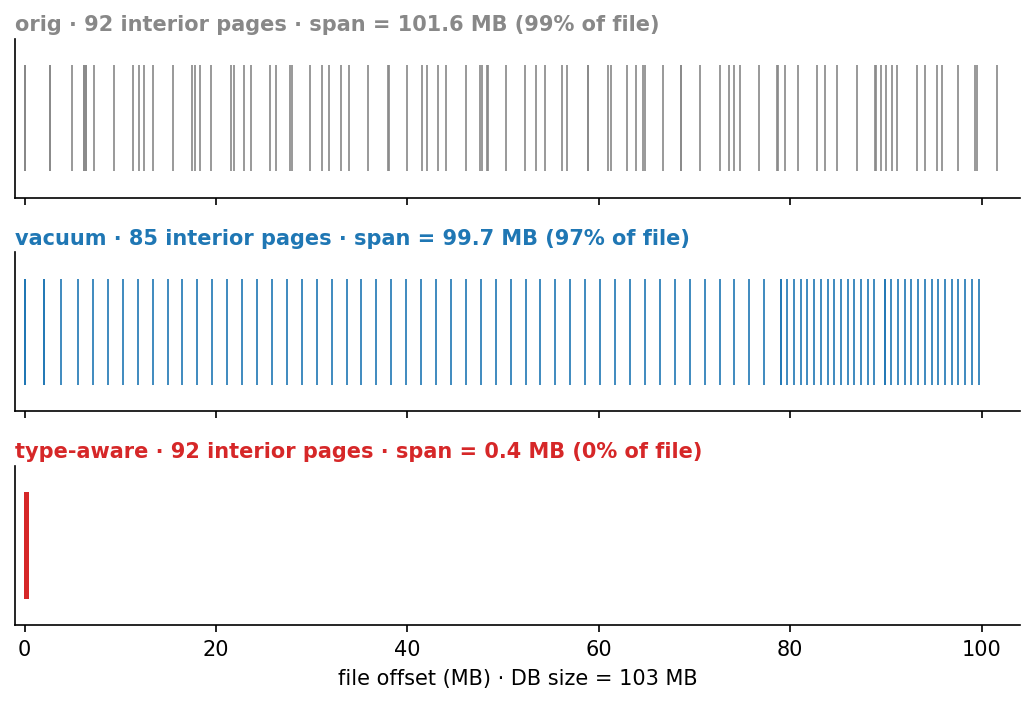
\includegraphics[width=1\linewidth]{figures/01_page_distribution.png}
\caption{Physical distribution of interior pages under the three layouts (file offset in MiB, 103 MiB file). \texttt{Default} and \texttt{Vacuum} scatter interior pages across the whole file, whereas \texttt{Clustered} confines them to the first 400 KB.}
\label{fig:layout-distribution}
\end{figure}

\subsection{Deployment Integration}\label{sec:deployment}

The two deployment models of Section~\ref{sec:cost-model} correspond to two integration points. The external-warmer model runs the prefetcher as a separate process, typically a sidecar, that opens the database file itself and therefore pays $t_\text{open}$ on every invocation (Eq.~\ref{eq:e2e_ext}). The warm-process model issues the hints from the application after its SQLite handle is open and before it serves the first request, reusing the handle (Eq.~\ref{eq:e2e_warm}). We advocate the latter for serverless keep-alive and edge-worker deployments, where the runtime stays resident across invocations.

When several processes on one node share a database file, for example multiple function instances, a single prefetch can serve all of them. With \texttt{PRAGMA mmap\_size} set to the file size, SQLite maps the file with \texttt{mmap(MAP\_SHARED)}, so pages one process brings into the OS page cache are visible to every process sharing the mapping. A private-cache configuration, in which each process reads through its own buffer with \texttt{read()}, serves as the baseline. Section~\ref{sec:eval-robustness} evaluates the shared cache together with the trade-off between re-warm cadence and freshness.

\section{Experimental Setup}\label{sec:setup}

\subsection{Platform}\label{sec:platform}

All workstation experiments run on one bare-metal commodity machine: an AMD Ryzen 9950X, 64 GB of memory, and a 2 TB NVMe Gen4 ×4 SSD, under Linux kernel 6.17. \texttt{read\_ahead\_kb} stays at its default of 128 KB (Section~\ref{sec:selection-delivery}), and CPU frequency pinning follows Section~\ref{sec:protocol}. The OpenWhisk deployment runs on a separate host described in Section~\ref{sec:setup-openwhisk}. Section~\ref{sec:discussion} discusses the limits of a single-machine platform.

\subsection{Reference Database}\label{sec:refdb}

The reference database has one table, \texttt{items(id INTEGER PRIMARY KEY, k1 INTEGER, k2 INTEGER, payload BLOB(100))}, with a secondary index on \texttt{(k1, k2)}. It holds 600,000 rows in 102.9 MiB (107{,}851{,}776 bytes) of 4 KB pages, whose interior and leaf composition Section~\ref{sec:btree} describes. \texttt{Default} and \texttt{Clustered} each contain 26,331 pages, and \texttt{Vacuum} contains 25,613. A 10$\times$ variant with 6,000,000 rows and 263,991 pages (about 1 GiB) serves the size-scaling experiment of Section~\ref{sec:eval-robustness}.

\subsection{Workloads}\label{sec:workloads}

Table~\ref{tab:workloads} lists the primary workloads. Three read-only workloads are measured for first-query latency and cover three access characteristics. Scattered-Zipf-100K issues point reads from a scrambled Zipfian distribution ($\alpha = 0.99$, following the profile of YCSB-C~\cite{Cooper2010}) over a 100,000-key active domain (ids 1 through 100,000), with a key permutation that scatters hot keys across the domain. Uniform-100K issues uniform point reads over the same domain and is the matched no-skew control. Tail-Mixed draws uniformly over a 20,000-key interval (ids 590,000 through 609,999) that straddles the maximum id of 600,000, so about half of its lookups are not-found probes that all descend to the rightmost leaf. Each read workload executes 100,000 operations. Scattered-Zipf-100K and Uniform-100K use the YCSB op-string format and reproduce the YCSB distributions rather than its sampling implementation\footnote{\url{https://github.com/ls4154/YCSB-cpp}}. Tail-Mixed has no YCSB counterpart. Mixed-Mutation Churn is a write-heavy mutation schedule that ages the database between measured probes in the churn experiment of Section~\ref{sec:eval-robustness} and is not itself latency-measured. We refer to every workload by its descriptive name throughout, which avoids confusion with the YCSB core workloads A to F.

\begin{table}[htbp]
\centering
\caption{Primary workloads. The three read workloads are latency-measured, and Mixed-Mutation Churn only ages the database between probes.}
\begin{tabular}{p{0.15\linewidth}p{0.35\linewidth}p{0.35\linewidth}}
\toprule
\textbf{Workload} & \textbf{Access pattern} & \textbf{Serverless scenario} \\
\midrule
Scattered-Zipf-100K & Zipfian point reads (skewed, permuted key space) & Function-local hot-key lookups, e.g., user configuration or cache keys \\
Uniform-100K & Uniform random point reads & Random-access point lookups, e.g., analytics point sampling over the key space \\
Tail-Mixed & Uniform point reads over ids 590,000 to 609,999, about half not-found and concentrated on the rightmost leaf & Existence / boundary checks, e.g., idempotency or deduplication probes against a high-key range \\
Mixed-Mutation Churn & Write-heavy mutation schedule (\emph{not} a measured workload) & Ages the database via writes, used only in the churn robustness experiments (Section~\ref{sec:eval-robustness}) \\
\bottomrule
\end{tabular}
\label{tab:workloads}
\end{table}

Three auxiliary workloads, all on \texttt{Default}, support specific controls. Tail-Hit draws a tail range of the same size as Tail-Mixed entirely within the key space (zero not-found) and isolates the not-found effect in Section~\ref{sec:eval-attribution}. Latest-Aging and Short-Scan Aging are deterministic reconstructions of the YCSB-D and YCSB-E semantics rather than official traces. Latest-Aging's read hotspot moves as keys are inserted, whereas Short-Scan Aging's is stationary, and the two drive the static-plan staleness experiment of Section~\ref{sec:eval-robustness}. None of the auxiliary workloads alters the baselines below.

The OpenWhisk deployment (Section~\ref{sec:setup-openwhisk}) additionally runs three native YCSB 0.17.0 traces over the full 600,000-key space: Scattered-Zipf-600K, Uniform-600K, and Hotspot-1\%-scattered, a workload-C read mix with Zipfian, uniform, and 1\% hotspot request distributions, the last with hot keys hashed across the physical key space. All three are pure-hit. Scattered-Zipf-600K and Uniform-600K are the external-validity counterparts of the controlled Scattered-Zipf-100K and Uniform-100K. Hotspot-1\%-scattered is a native hotspot regime with no controlled counterpart, and is not equated with Tail-Mixed. These three are used only in Section~\ref{sec:eval-portability}, which also carries Tail-Mixed and Tail-Hit across both platforms.

Under \texttt{Default}, the median cold first-query latencies are 500~\textmu s for Scattered-Zipf-100K, 732~\textmu s for Uniform-100K, and 1067~\textmu s for Tail-Mixed, against 1 to 3 µs with a warm cache. These cold values are the denominators for every improvement reported in Section~\ref{sec:evaluation}. The workload traces are published with the artifact, checksummed, together with the generator that drives the 10-seed analysis of Section~\ref{sec:stats}.

\subsection{OpenWhisk Portability Deployment}\label{sec:setup-openwhisk}

The portability experiment of Section~\ref{sec:eval-portability} runs the same prefetch toolchain as an action inside Apache OpenWhisk on a separate commodity x86 host with its own consumer NVMe SSD and a different Linux kernel. The action loads the \texttt{Default} reference database (26{,}331 pages) and issues hints through the same unprivileged interfaces (\texttt{mmap, madvise}) as on the workstation, with no kernel, firmware, or runtime modification. Because host and runtime differ together, the deployment tests deployability and relative effectiveness rather than hardware portability, and absolute microseconds are never compared with the workstation.

Each measured invocation is one arm of an A/B pair, a same-condition baseline arm and a strategy arm, scheduled in a block-union paired design with position balancing. Each arm opens a fresh handle, so the measurement is a per-invocation first query rather than either deployment boundary of Section~\ref{sec:cost-model}. The comparison quantity is the relative first-query reduction $R = (\mathit{fq}_{\mathrm{base}} - \mathit{fq}_{\mathrm{strat}})/\mathit{fq}_{\mathrm{base}}$, the only quantity compared across platforms. Seven frozen campaigns comprise 5{,}756 invocations and 2{,}878 pairs. Effect estimates are never pooled across campaigns, and the campaigns together cover all 65 strategy-workload cells the workstation ran: 55 first-query cells and 10 delivery-order cells.

\section{Evaluation}\label{sec:evaluation}

Our evaluation answers three questions. \textbf{RQ1}: does a lower first-query latency imply a faster cold start? Sections~\ref{sec:eval-fq} and~\ref{sec:eval-tradeoff} show that it does not, because charging delivery cost can reverse the first-query ranking. \textbf{RQ2}: under critical-path cost accounting, what should be prefetched? Section~\ref{sec:eval-attribution} shows that a small coverage set suffices: interior-navigation coverage is the robust default, hot leaves help only under an independently verified hotspot, and at matched footprint a type-aware selector does not beat a frequency-ranked dump. \textbf{RQ3}: do the end-to-end conclusions survive workload and system variation, and does first-query effectiveness survive a FaaS runtime? Section~\ref{sec:eval-robustness} tests the former across six robustness axes on the workstation, and Section~\ref{sec:eval-portability} tests the latter on OpenWhisk. Section~\ref{sec:eval-guidance} distills the results into deployment guidance.

\subsection{First-Query Gains and Workload-Dependent Ceilings}\label{sec:eval-fq}

We first report first-query latency alone, before charging preprocessing in Section~\ref{sec:eval-tradeoff}. Against the cold baselines of Section~\ref{sec:workloads} (500, 732, and 1067 \textmu s), Dump reaches the lowest first-query latency on every workload: 99 \textmu s on Scattered-Zipf-100K ($-80\%$), 100 \textmu s on Uniform-100K ($-86\%$), and 94 \textmu s on Tail-Mixed ($-91\%$). Judged by this metric alone, Dump wins outright. The targeted strategies reach $-27\%$ to $-83\%$, with a ceiling that depends on the workload (Table~\ref{tab:ceiling} and Figure~\ref{fig:firstq-bars}).

The ceiling has a structural explanation. At first-query time every page is cold, and interior prefetching removes the interior faults but leaves the first leaf fault. On Scattered-Zipf-100K the interior skeleton alone captures most of the benefit ($-27\%$ to $-28\%$), and adding leaves yields diminishing returns: \texttt{Skel+500} reaches $-64\%$ and Dump $-80\%$. On Uniform-100K there is no hot set, every query hits a cold leaf, and interior-only prefetching is capped at $-44\%$, with only the full dump going further, to $-86\%$. On Tail-Mixed the interior-only ceiling is $-38\%$, but \texttt{Skel+10} reaches $-83\%$ because about half the queries are not-found probes that descend to the same rightmost leaf, which \texttt{Skel+10} includes. This is a property of the key range rather than of tail reads in general, as Section~\ref{sec:eval-attribution} confirms with a pure-hit control.

The offset-ordered structural strategy \texttt{Skel-N} depends on both workload and layout. On Scattered-Zipf-100K and Uniform-100K the first five interior pages already reach the plateau ($-27\%$ to $-28\%$ and $-44\%$), and further interiors add nothing. Tail-Mixed needs nearly all 92, because the interiors covering its high-key range sit mid-file and offset-order selection reaches them only when N spans the whole set. A single page ($N = 1$) is counter-productive on Scattered-Zipf-100K, where \texttt{madvise} dispatch overhead exceeds the coverage gain and first-query latency is $31\%$ worse than the same-batch baseline, and only marginally helpful on the other two workloads. The shape of the N-sweep is consistent across the hotspot variants in our artifact.

Figure~\ref{fig:firstq-bars} plots each strategy's paired first-query reduction against its same-batch baseline. \texttt{Dump} leads on every workload, and \texttt{Skel+10} on Tail-Mixed is the largest targeted reduction. Section~\ref{sec:eval-tradeoff} revisits this ranking with end-to-end accounting.

\begin{table}[htbp]
\centering
\small
\renewcommand{\arraystretch}{1.2}
\caption{First-query improvement ceiling by workload. Ceiling is the best interior-only reduction (\texttt{Skel} or \texttt{Skel-92}), and the second column is the best reduction with hot leaves or the full dump.}
\begin{tabular}{>{\raggedright\arraybackslash}p{0.28\linewidth}
                >{\centering\arraybackslash}p{0.18\linewidth}
                >{\raggedright\arraybackslash}p{0.43\linewidth}}
\toprule
\textbf{Workload} & \textbf{Ceiling} & \textbf{With hot leaves / full dump} \\
\midrule
Scattered-Zipf-100K & $-28\%$ & \texttt{Skel+500}: $-64\%$, \texttt{Dump}: $-80\%$ \\
Uniform-100K        & $-44\%$ & \texttt{Dump}: $-86\%$ \\
Tail-Mixed          & $-38\%$ & \texttt{Skel+10}: $-83\%$, \texttt{Dump}: $-91\%$ \\
\bottomrule
\end{tabular}
\label{tab:ceiling}
\end{table}

\begin{figure*}[htbp]
\centering
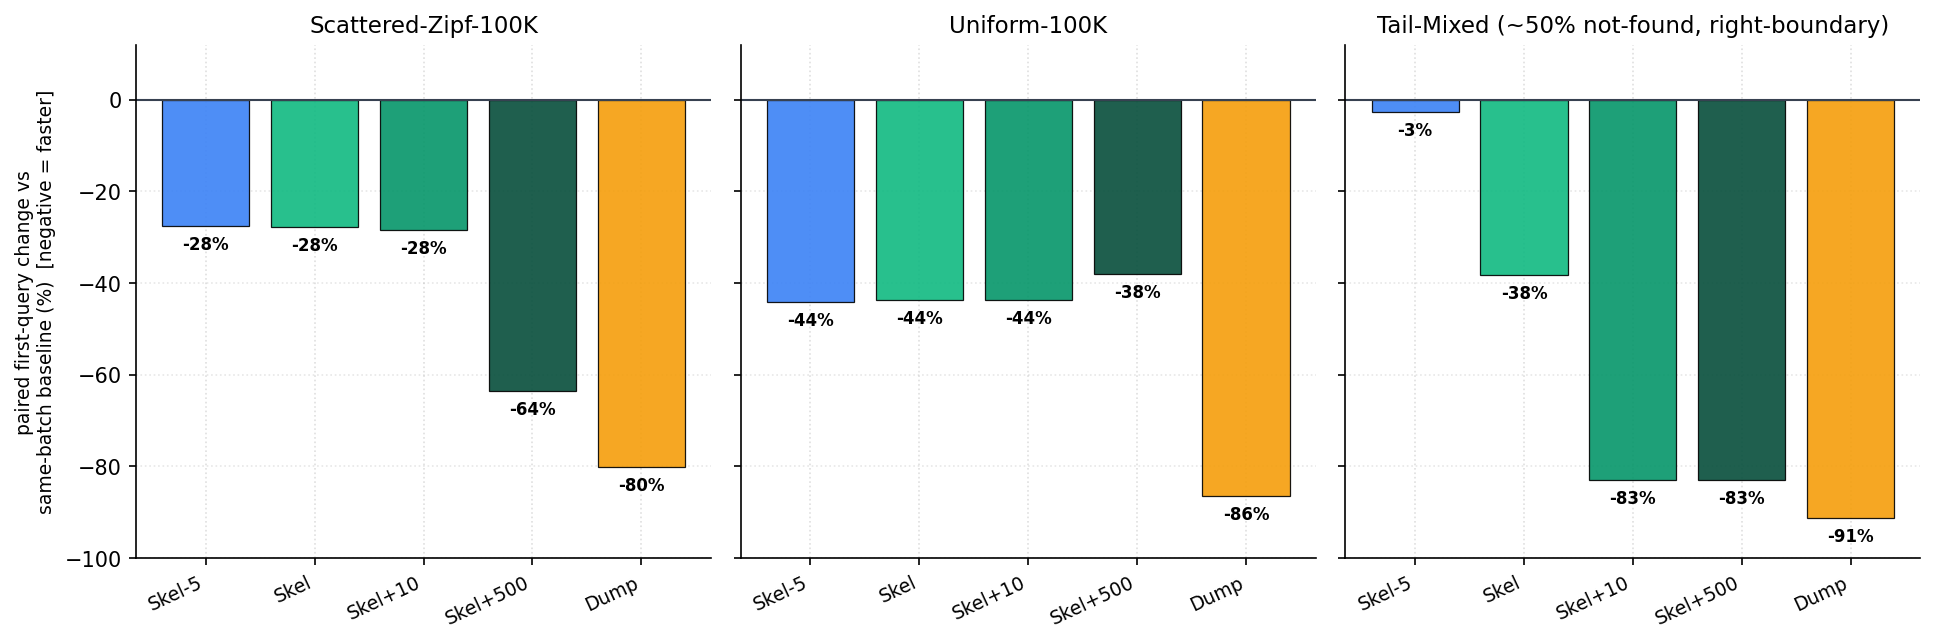
\includegraphics[width=\textwidth]{figures/13_strategy_firstq_bars.png}
\caption{Paired first-query reduction by strategy and workload (median change versus each strategy's same-batch baseline, negative is faster). All cells are from one batch under the corrected tie-break. \texttt{Dump} attains the largest reduction on every workload ($-80\%$ to $-91\%$), which Figure~\ref{fig:e2e-stacked} shows does not translate into end-to-end wins.}
\label{fig:firstq-bars}
\end{figure*}

\subsection{The Preprocessing Trade-off}\label{sec:eval-tradeoff}

First-query latency excludes the cost of the prefetch itself. Table~\ref{tab:overhead} decomposes that cost per strategy. The cold-open cost $t_\text{open}$ is a per-layout constant, about 179 \textmu s in the main batch and independent of strategy and workload. Because the two deployment models of Section ~\ref{sec:cost-model} differ only by $t_{\text{open}}$, it shifts both models' zero points equally ($e2e_{\text{ext}} - (\text{baseline} + t_{\text{open}}) = e2e_{\text{warm}} - \text{baseline}$) and never decides a within-model comparison. The delivery cost $t_\text{deliver}$ scales with the prefetch set: 68 to 124 \textmu s for \texttt{Skel-5}, \texttt{Skel}, and \texttt{Skel+10}, 0.5 to 0.85 ms for \texttt{Skel+500}, and 0.8 to 7 ms for \texttt{Dump}, which pays about 7 ms on the two 100K workloads and 0.80 ms on Tail-Mixed.

Charging $t_\text{deliver}$ reverses the ranking of Section~\ref{sec:eval-fq}. Table~\ref{tab:e2e-ac} gives end-to-end latency under both models for the main batch, and Figure~\ref{fig:e2e-stacked} stacks first query and delivery for the warm-process model. \texttt{Dump}, the first-query winner, is the end-to-end loser on the broad workloads: on Scattered-Zipf-100K its 7 ms delivery dwarfs its 401 \textmu s first-query gain, regressing the warm-process cold start by $+1330\%$ (7148 versus 500 \textmu s) and the external-warmer cold start by $+1366\%$, and on Uniform-100K it regresses by $+882\%$. Tail-Mixed, whose working set is only 1.8 MB, is the sole exception at $-20\%$ (cross-seed $-10\%$, robust). Over-provisioning leaves fails the same way in miniature: \texttt{Skel+500} regresses by $+106\%$ and $+79\%$ on the two broad workloads.

The frugal strategies \texttt{Skel} and \texttt{Skel+10} improve warm-process latency on all three workloads. The robust general result is \texttt{Skel} at roughly $25\%$ to $30\%$ across the pure-hit workloads (cross-seed, Section~\ref{sec:eval-robustness}). Tail-Mixed \texttt{Skel+10} shows a larger single-instantiation $-75\%$ (1067 to 262 \textmu s), but Section~\ref{sec:eval-attribution} shows this is driven by the not-found rightmost-leaf concentration and is bimodal across seeds with a mean of $-55\%$. The single-instantiation wins of \texttt{Skel-5} do not survive cross-seed validation: tie on Scattered-Zipf-100K, directional toward regression on Uniform-100K, and robustly worse on Tail-Mixed (Table~\ref{tab:e2e-ac}).

The deployment model decides whether prefetching pays at all. In the external-warmer model the cold open consumes the benefit on the fast workloads (\texttt{Skel} on Scattered-Zipf-100K: $+25\%$), whereas in the warm-process model the same strategies win consistently. Three conclusions follow. Minimizing first-query latency does not guarantee a faster cold start, because delivery cost can dominate the critical path. The deployment model determines the verdict, and the warm-process model we advocate is where targeted prefetch wins. The open cost is a deployment constant rather than a prefetch tax: it shifts the zero point between models but never their internal ranking.

\begin{table}[htbp]
\centering
\caption{Preprocessing cost by strategy, from a separate overhead-decomposition batch whose open medians (193 to 222 \textmu s) differ from the main batch's 179 \textmu s by cross-batch drift. $t_\text{open}$ is constant per layout, and $t_\text{deliver}$ scales with set size.}
\begin{tabular}{l r r l}
\toprule
\textbf{Strategy} & $t_{\text{open}}$ & $t_{\text{deliver}}$ & \textbf{Dominant term} \\
\midrule
\texttt{Skel-5} & $\sim$193 \textmu s & $\sim$68 \textmu s & open \\
\texttt{Skel-92} & $\sim$194 \textmu s & $\sim$190 \textmu s & balanced \\
\texttt{Skel} & 194--222 \textmu s & 68--110 \textmu s & open \\
\texttt{Skel+10} & 193--222 \textmu s & 80--124 \textmu s & open \\
\texttt{Skel+500} & $\sim$220 \textmu s & 0.5--0.85 ms & deliver \\
\texttt{Dump} & $\sim$220 \textmu s & 0.8--7 ms & deliver \\
\bottomrule
\end{tabular}
\label{tab:overhead}
\end{table}

\begin{table*}[htbp]
\centering
\small
\setlength{\tabcolsep}{3pt}
\renewcommand{\arraystretch}{1.25}
\newcolumntype{L}[1]{>{\hsize=#1\hsize\raggedright\arraybackslash}X}
\newcolumntype{C}[1]{>{\hsize=#1\hsize\centering\arraybackslash}X}
\newcolumntype{R}[1]{>{\hsize=#1\hsize\raggedleft\arraybackslash}X}
\caption{End-to-end latency under the external-warmer (\texttt{e2e\_ext}) and warm-process (\texttt{e2e\_warm}) models, main batch, \texttt{Default} layout, asynchronous delivery. Every value in this table and in Tables~\ref{tab:ablation},~\ref{tab:competitive} and~\ref{tab:seeds} comes from one 10-seed batch measured in a single contiguous window under the corrected tie-break. The $\text{e2e}_{\text{ext}}$ column adds a cold open whose median varies by about 30~\textmu s with the prefetched set and across batches, so its absolute values carry that uncontrolled term. \texttt{Skel+10} and \texttt{Skel+500} are plotted in Figure~\ref{fig:e2e-stacked}. Percentages are single-instantiation paired improvements, and verdicts are the cross-seed classifications of Section~\ref{sec:eval-robustness}.}
\begin{tabularx}{\textwidth}{L{0.5} *{4}{C{0.65}} L{2.5}}
\toprule
\multirow{2}{*}{\textbf{Strategy}} & 
\multicolumn{2}{c}{\shortstack{\textbf{Scattered-Zipf-100K}\\(baseline 500\,\textmu s)}} & 
\multicolumn{2}{c}{\shortstack{\textbf{Tail-Mixed}\\(baseline 1067\,\textmu s)}} & 
\multirow{2}{*}{\textbf{Cross-seed verdict}} \\
\cmidrule(lr){2-3} \cmidrule(lr){4-5}
& $\text{e2e}_{\text{ext}}$ & $\text{e2e}_{\text{warm}}$ & $\text{e2e}_{\text{ext}}$ & $\text{e2e}_{\text{warm}}$ & \\
\midrule
Baseline        & 500            & 500            & 1067          & 1067          & n/a \\
\texttt{Skel-5} & 581 (+16\%)   & 433 ($-$13\%)  & 1291 (+21\%)  & 1108 (+4\%)   & Scattered-Zipf-100K: \textit{tie}, Tail-Mixed: \textit{robust} (worse) \\
\texttt{Skel}   & 624 (+25\%)   & 446 ($-$11\%)  & 909 ($-$15\%) & 728 ($-$32\%) & Scattered-Zipf-100K: \textit{robust} ($-$27\%), Tail-Mixed: \textit{robust} ($-$37\%) \\
\texttt{Dump}   & 7325 (+1366\%) & 7148 (+1330\%) & 1000 ($-$6\%)  & 856 ($-$20\%) & Scattered-Zipf-100K: \textit{robust} (worse), Tail-Mixed: \textit{robust} ($-$10\%) \\
\bottomrule
\end{tabularx}
\label{tab:e2e-ac}
\end{table*}

\begin{figure*}[htbp]
\centering
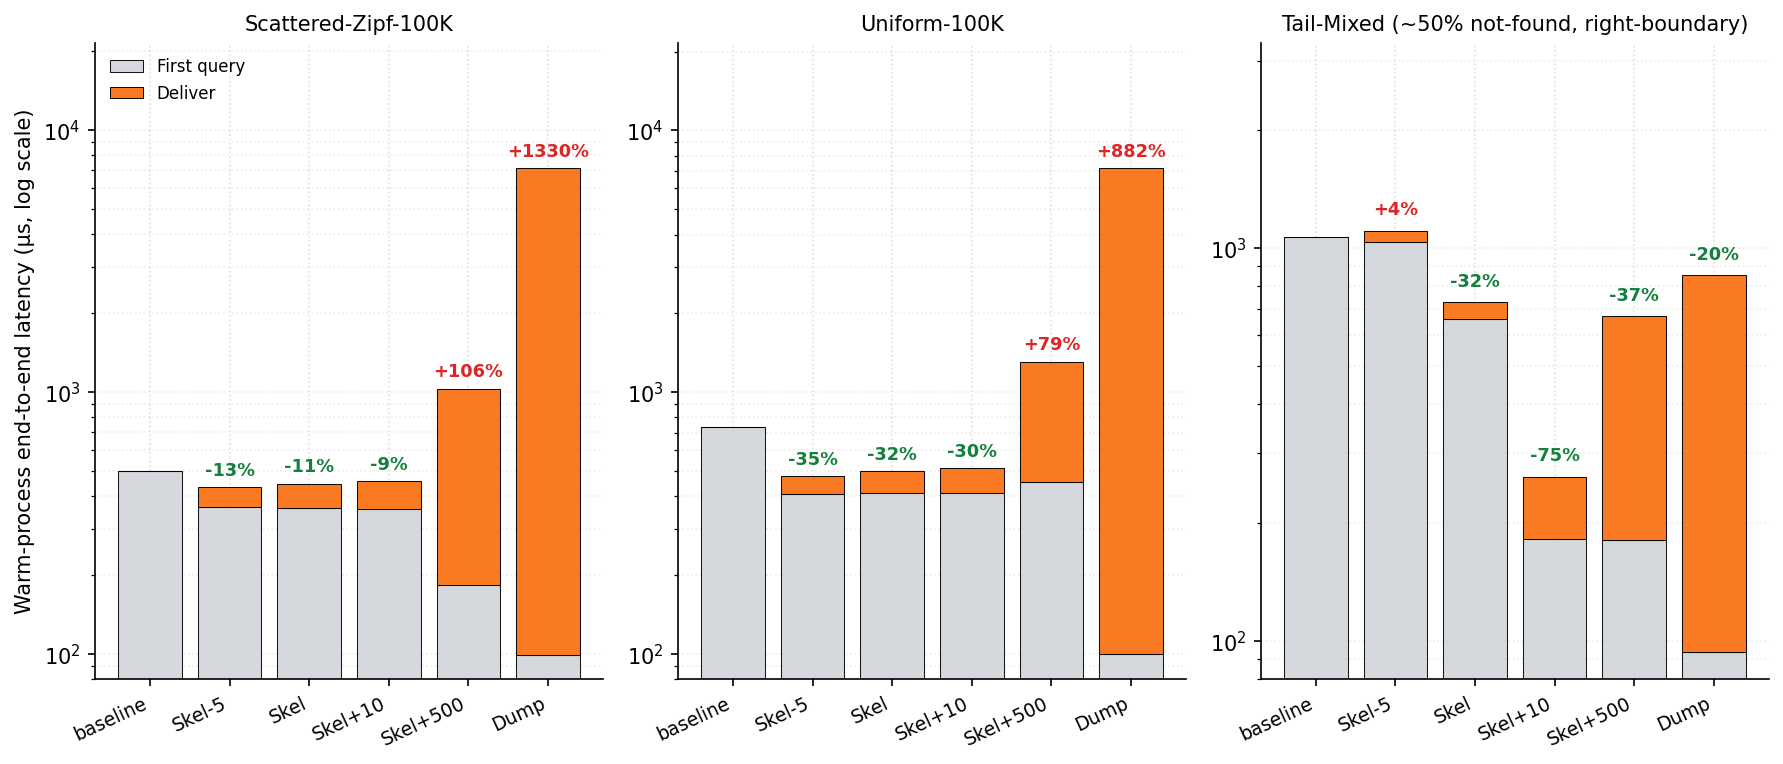
\includegraphics[width=\textwidth]{figures/14_strategy_endtoend_stacked.png}
\caption{Warm-process end-to-end decomposition, same batch as Figure~\ref{fig:firstq-bars}. Each bar stacks first query and delivery, so its height is \texttt{e2e\_warm}. Labels are paired changes versus the dashed same-workload baseline. \texttt{Dump} regresses by $+1330\%$ and $+882\%$ on the broad workloads and is the exception on Tail-Mixed ($-20\%$), \texttt{Skel+500} regresses by $+106\%$ and $+79\%$, and \texttt{Skel} sits below baseline on all three. The \texttt{Skel-5} improvements are single-instantiation only (Table~\ref{tab:e2e-ac}).}
\label{fig:e2e-stacked}
\end{figure*}

\subsection{Attribution: Ablation and Competitive Baselines}\label{sec:eval-attribution}

\textbf{Ablation of the two levers.} The large Tail-Mixed result of Section~\ref{sec:eval-tradeoff} combines page-type and access-frequency selection. We separate them with an exact decomposition of the \texttt{Skel+10} set into four arms: \texttt{Skel} (resident interiors only), \texttt{leaf\_freq\_K10} (the top-10 leaves by access count only), \texttt{leaf\_rand\_K10} (10 leaves of the same type drawn uniformly at random, a control that matches page count and type and differs only in selection criterion), and \texttt{Skel+10} (the union of the first two). This attribution required fixing an estimator artifact. Our original leaf ranking broke frequency ties by first-seen order, which on a tied-count workload favored the earliest-observed leaves, the ones the measured first query touches, so they leaked into the set. We replaced it with a trace-order-independent tie-break (frequency descending, then page number ascending) and re-measured every affected cell in one same-batch 10-seed rerun with paired baselines. Numbers in this subsection are from that rerun unless stated otherwise, so they are cross-seed means and differ from the single-instantiation values of Sections~\ref{sec:eval-fq} and~\ref{sec:eval-tradeoff}.

Table~\ref{tab:ablation} gives the corrected ablation on Tail-Mixed. \texttt{Skel} alone is $-44\%$ first-query and $-37\%$ end-to-end and is the only robust contributor. \texttt{leaf\_rand\_K10} is net-harmful end-to-end ($+6\%$): extra leaves without a hotspot cost delivery for no coverage. \texttt{leaf\_freq\_K10} alone is $-4\%$ end-to-end with a CI crossing zero, a tie, and its pre-fix $-40\%$ was almost entirely first-op leakage. \texttt{Skel+10} reaches $-64\%$ first-query and $-55\%$ end-to-end but is bimodal across seeds, as explained below. The hierarchy is therefore asymmetric: interior coverage is the robust lever and the prerequisite for any leaf benefit, since a leaf is useless while its path is uncached, and leaf frequency is a conditional add-on. The 10-seed sweep of Section~\ref{sec:eval-robustness} characterizes the other workloads: on Uniform-100K the entire gain is the skeleton (\texttt{Skel} $-26\%$), and on Scattered-Zipf-100K the frequency lever adds a robust bonus beyond it (\texttt{Skel} $-27\%$ to \texttt{Skel+10} $-38\%$), consistent with its Zipfian skew.

\textbf{Why the Tail-Mixed result is narrow.} About half of Tail-Mixed's lookups are not-found probes, and every one descends the right edge to the same rightmost leaf, an extreme key-range-induced hotspot. The corrected \texttt{Skel+10} result is accordingly bimodal: about $-71\%$ when the measured first query is itself a not-found probe and about $-32\%$, the interior-skeleton regime, when it is a hit, for a mean of $-55\%$. On the matched pure-hit control Tail-Hit, \texttt{Skel+10} returns to about $-27\%$, statistically matching \texttt{Skel} ($-28.5\%$) and a footprint-matched frequency dump ($-30.6\%$). Once the not-found concentration is removed, leaf frequency adds nothing beyond the skeleton. We report the Tail-Mixed number as a scoped, mechanism-specific result.

\textbf{Competitive baselines.} To test whether \texttt{Dump} is a weak baseline, we port the
selection cores of two prior systems (Section~\ref{sec:buffer-warming}) onto our substrate and
charge them the same way. \texttt{Dump} is the full-working-set core of InnoDB's buffer-pool
dump and load. \texttt{Dump-N} is a frequency-ranked partial dump in the spirit of Pre-Buffer.
It replays each query's root-to-leaf traversal, counts page visits, and dumps the top $N$ pages
for $N$ in {14, 28, 100, 500, full}. We reproduce only the selection, not the off-critical-path
orchestration of either system. Table~\ref{tab:competitive} reports warm-process end-to-end
results under both delivery modes. Under per-page delivery, end-to-end latency worsens
monotonically with dump footprint. The full dump regresses by $+770\%$ on Scattered-Zipf-100K
and $+724\%$ on Uniform-100K, so the problem is delivery volume rather than the dump mechanism.
At matched footprint a small ranked dump ties \texttt{Skel+10} on every workload
(Scattered-Zipf-100K $-31\%$ versus $-38\%$, Uniform-100K $-26\%$ versus $-25\%$, Tail-Mixed
$-57\%$ versus $-57\%$, all with overlapping CIs). Explicit page typing and frequency ranking
recover a similar page set, so page-type knowledge earns its place as an interpretable coverage
guarantee rather than as a faster selector.

\textbf{Delivery mechanism.} Selection and delivery are separate axes, and the fair test
charges every arm the stronger mechanism. Window-chunked delivery cuts the full dump's delivery
term from 7.0 ms to 1.9 ms on the two 100K-key workloads, from 0.76 ms to 0.22 ms on Tail-Mixed
and from 1.40 ms to 0.42 ms on the pure-hit control, moving it from $+770\%$ to $+150\%$ on
Scattered-Zipf-100K, from $+724\%$ to $+137\%$ on Uniform-100K, from $-9\%$ to $-66\%$ on
Tail-Mixed, and from $+72\%$ to $-41\%$ on the pure-hit control. The same mechanism moves
\texttt{Skel+10} only from 98 to 33 \textmu s, because its ranges already sit at or below the
window. That asymmetry is the finding. A mechanism that makes delivery cheap helps whoever was
delivering the most, so it rewrites the baseline far more than it rewrites our own arms. The
consequence is a split verdict. On the two broad workloads targeted selection still wins by a
wide margin under the same mechanism, $-45\%$ and $-33\%$ against $+150\%$ and $+137\%$, because
a 17.7 MB transfer still costs 1.9 ms for pages no query touches. On the two tail workloads,
whose working sets are small enough that the transfer is cheap once chunked, the full dump
overtakes us, $-66\%$ against our $-62\%$ on Tail-Mixed and $-41\%$ against our $-35\%$ on the
pure-hit control. We therefore report window-chunked delivery as the deployable default, and we
state the scope of the targeted-prefetch claim as workloads whose working set is large relative
to what a cold start can afford to transfer.

\textbf{Delivery order.} libprefetch's contribution is ordering at a fixed set (Section~\ref{sec:os-prefetch}). We deliver the same 18 MB working set as \texttt{Dump} in ascending file-offset order (\texttt{LP-sorted}) and shuffled (\texttt{LP-shuf}). On NVMe the ordering effect survives only in the synchronous delivery term, where \texttt{pread} is $10$ to $16 \times$ slower shuffled than sorted ($15.6\times$, $15.1\times$, and $10.5\times$ on the three workloads), and first-query latency is unchanged because both arms deliver the same pages. Asynchronous \texttt{fadvise} dispatch shows no ordering effect (delivery ratio about 1.0). Delivery scheduling is therefore orthogonal to set selection.

\textbf{Learned prefetching.} In the lineage of Chen et al.~\cite{Chen2021}, we train a first-order Markov page-transition model that computes finite-horizon expected visits from the root and prefetches the top $N$, evaluated with leave-one-seed-out cross-validation over the 10 seeds. At matched footprint it reduces first-query latency by $-39.6\%$, $-36.6\%$, and $-65.4\%$ on the three workloads, every CI excluding zero. It ties frequency ranking and targeted prefetch on Uniform-100K and Tail-Mixed, and on Scattered-Zipf-100K it reaches about $-40\%$ against about $-51\%$ for the same-budget arms, with overlapping CIs. The learned model shows no advantage over the simpler frequency-ranked baseline.

\textbf{Physical layout.} Measured in the same batch as Table~\ref{tab:e2e-ac}, the best
warm-process end-to-end latency for \texttt{Default} versus \texttt{Clustered} is 414 versus
507 \textmu s on Scattered-Zipf-100K, 475 versus 670 \textmu s on Uniform-100K, and 253 versus
302 \textmu s on Tail-Mixed. The layout interacts with the selection strategy rather than with
prefetch as a whole. For the strategies we recommend, \texttt{Clustered} is worse and the effect
is consistent across instantiations. \texttt{Skel+10} is $1.07\times$ slower under
\texttt{Clustered} on Scattered-Zipf-100K on all 10 seeds and $1.12\times$ slower on Tail-Mixed
on 8 of 10. For pure interior selection the sign reverses. \texttt{Skel-92} on Tail-Mixed is
$0.88\times$ under \texttt{Clustered} on all 10 seeds, because clustering raises the interior
page count the skeleton captures from 4 pages to 48. The synchronous first-query floor is
unchanged by layout at 183 versus 181 \textmu s, so the layout changes which pages a strategy
finds rather than how fast they can be delivered. We therefore recommend \texttt{Default} for
the strategies of Section~\ref{sec:strategy}, and note \texttt{Clustered} as the better pairing
in the one case where only structural selection is available and the workload is tail-heavy.
The \texttt{.dbi} side file of Section~\ref{sec:serverless-coldstart} reaches the same
conclusion by copying navigation pages instead of reordering them.

\begin{table}[htbp]
\centering
\caption{Corrected ablation on Tail-Mixed, 10-seed means with $95\%$ bootstrap CIs. \texttt{leaf\_rand\_K10} matches \texttt{leaf\_freq\_K10} in page count and type and differs only in selection criterion.}
\begin{tabular}{l c r r}
\toprule
\textbf{Arm} & \textbf{Pages} & \textbf{First-query $\Delta\%$} & \textbf{$\text{e2e}_{\text{warm}}$ $\Delta\%$} \\
\midrule
\texttt{Skel} & 4 & $-44\%$ $[-47, -41]$ & $-37\%$ (robust) \\
\texttt{leaf\_rand\_K10} & 10 & $-2\%$ $[-4.0, -0.1]$ & $+6\%$ (worse) \\
\texttt{leaf\_freq\_K10} & 10 & $-12\%$ $[-22, -1]$ & $-4\%$ (tie) \\
\texttt{Skel+10} & 14 & $-64\%$ $[-76, -52]$ & $-55\%$ (bimodal) \\
\bottomrule
\end{tabular}
\label{tab:ablation}
\end{table}

\begin{table*}[htbp]
\centering
\caption{Frequency-ranked partial dump versus targeted prefetch, warm-process end-to-end, 10-seed means with $95\%$ bootstrap CIs. All twelve cells are from the same 10-seed batch as Tables~\ref{tab:e2e-ac},~\ref{tab:ablation} and~\ref{tab:seeds}, so the columns are mutually comparable.}
\begin{tabular}{l l r r r}
\toprule
\textbf{Arm} & \textbf{Footprint} & \textbf{Scattered-Zipf-100K} & \textbf{Uniform-100K} & \textbf{Tail-Mixed} \\
\midrule
\texttt{Skel+10} (targeted) & 14--28 pages & $-38\%$ $[-52, -24]$ & $-26\%$ $[-32, -17]$ & $-55\%$ $[-68, -43]$ \\
\texttt{Dump-14} (ranked) & 14 pages & $-31\%$ $[-42, -22]$ & $-27\%$ $[-34, -17]$ & $-55\%$ $[-67, -43]$ \\
\texttt{Dump-500} (ranked) & 500 pages & $+83\%$ $[+35, +155]$ & $+44\%$ $[+26, +60]$ & $-9\%$ $[-13, -5]$ \\
\texttt{Dump} (full dump) & $\sim$4400 pages & $+767\%$ $[+677, +903]$ & $+722\%$ $[+641, +827]$ & $-10\%$ $[-14, -5]$ \\
\bottomrule
\end{tabular}
\label{tab:competitive}
\end{table*}

\subsection{Robustness}\label{sec:eval-robustness}

We test the headline conclusions along six axes, each on its own batch, so comparisons are within-axis and verdicts use the classifications of Section~\ref{sec:stats}.

\textbf{Workload instantiation.} Table~\ref{tab:seeds} reports cross-seed warm-process improvements from the 10-seed sweep. The robust general result is the interior skeleton: \texttt{Skel} improves warm-process latency by $-27\%$ on Scattered-Zipf-100K, $-26\%$ on Uniform-100K, and $-28.5\%$ on Tail-Hit, all with CIs excluding zero. The larger figures belong to Scattered-Zipf-100K \texttt{Skel+10} at $-38\%$, a skew bonus, and to \texttt{Tail-Mixed Skel} at $-37\%$, inflated by the not-found hotspot. \texttt{Tail-Mixed Skel+10} is $-55\%$ but bimodal (Section~\ref{sec:eval-attribution}). \texttt{Skel-5} does not survive: tie on Scattered-Zipf-100K ($-5\%$, 6 of 10 seeds) and directional toward regression on Uniform-100K, where 8 of 10 seeds worsen (median $+4\%$) and two strongly improving seeds pull the mean to $-2\%$. Structural prefetching without access observation is unreliable. The sweep also shows why single instantiations mislead: the main batch drew a Scattered-Zipf-100K instance with an unusually cheap first query (500 \textmu s against a cross-seed median of 886 \textmu s), so its \texttt{Skel+10} estimate of $-9\%$ understates the cross-seed $-38\%$, and it overstated Uniform-100K \texttt{Skel-5} at $-35\%$ against a cross-seed $-2\%$.

\textbf{Memory pressure.} Serverless platforms cap per-function memory through cgroup \texttt{ MemoryMax}. We sweep the cap from 16 MB to 6 MB, $0.92\times$ to $0.35\times$ the working set of the two 100K workloads (Figure~\ref{fig:ram}). The five targeted strategies, with sets of 20 KB to 2 MB, keep $100\%$ delivery and flat first-query latency at every cap, because their sets are far below the cap. Dump, whose 17.7 MB set is the working set, loses delivery linearly ($100\%$ to $20\%$), and its first-query latency jumps from 98 \textmu s to the cold baseline as soon as delivery falls below $100\%$: the cache dump degrades all at once rather than gracefully. Tail-Mixed's 1.8 MB working set is below the measurable pressure floor, so its robustness on this axis follows from set size and is not measured.

\textbf{Write churn.} We apply 50,000 mutations in 10 rounds and measure a frozen t = 0 set at 11 checkpoints. This batch predates the tie-break fix, so we use it only for within-batch flatness, not for effect magnitude. Under a stationary read hotspot the frozen set shows no systematic drift: Tail-Mixed \texttt{Skel+10} stays at 82 to 89 \textmu s across checkpoints (one transient spike at checkpoint 4) against a baseline near 580 \textmu s, and Uniform-100K is likewise flat. Write churn perturbs layout but not the read hotspot, so no refresh is needed here. A moving hotspot is the next axis.

\textbf{Static-plan staleness.} Latest-Aging moves the read hotspot as keys are inserted, and Short-Scan Aging keeps it stationary (Section~\ref{sec:workloads}). A frozen t = 0 plan is replayed at 11 checkpoints over 10 seeds. Under Latest-Aging the frequency plan \texttt{Skel+10}-static erodes from $-50\%$ to $-33\%$ first-query benefit as the hotspot moves away, whereas the structural plan \texttt{Skel-92}-static holds at $-53\%$ throughout. Under Short-Scan Aging both stay flat ($-53\%$ to $-55\%$ and $-53\%$ to $-51\%$). A static frequency plan is safe only while the hotspot is stationary. When it moves, structural coverage is the durable choice.

\textbf{Cadence and shared cache.} With \texttt{mmap(MAP\_SHARED)} one background warmer re-warms the set for every process sharing the page cache. At a 1 s or 5 s cadence, first-query latency holds at 26 and 29 \textmu s. At 30 s or never it regresses to 281 to 305 \textmu s, near baseline. The cadence trades warmth for I/O and CPU, and the operator picks a point from the workload's query interval.

\textbf{Database size.} On the $10\times$ database (Section~\ref{sec:refdb}), measured in the
same batch as Table~\ref{tab:e2e-ac}, 28 of 36 workload-strategy cells keep their direction.
Targeted prefetch does not merely hold at scale, it improves. \texttt{Skel} moves from $-27\%$
to $-52\%$ on Scattered-Zipf-100K, from $-26\%$ to $-52\%$ on Uniform-100K, and from $-37\%$ to
$-50\%$ on Tail-Mixed, and \texttt{Skel+10} moves from $-57\%$ to $-80\%$ on Tail-Mixed. A
larger database raises the cold baseline without enlarging a skeleton whose delivery cost grows
only $1.07\times$. Of the eight direction changes, five are large-footprint arms that regress at
the reference size and become neutral at $10\times$, including \texttt{Skel+500} at $+81\%$ to
$-3\%$ on Scattered-Zipf-100K, because the rising baseline absorbs a delivery cost that grows
more slowly than it does. The one substantive degradation is the full dump on Tail-Mixed, whose
resident working set doubles and whose delivery cost grows $2.05\times$, from 749 to 1534
\textmu s, turning a $-9\%$ win into a $+29\%$ regression. \texttt{Skel-92} on Tail-Mixed also
loses its win, from $-21\%$ to parity. The delivery trap therefore worsens with size for the
unranked full dump, and frugal coverage does not.

\begin{table*}[htbp]
\centering
\caption{Cross-seed validation of warm-process improvements. Single-workload values are main-batch point estimates, cross-seed values are 10-seed bootstrap means with $95\%$ CIs, and verdicts follow Section~\ref{sec:methodology} with the fraction of seeds agreeing in sign. †Tail-Mixed \texttt{Skel+10} is bimodal: about $-71\%$ when the first query is a not-found probe and about $-32\%$ when it is a hit.}
\begin{tabular}{l c c c}
\toprule
\textbf{Cell} & \textbf{Single workload} & \textbf{Cross-seed mean} & \textbf{Verdict} \\
\midrule
Tail-Mixed \texttt{Skel+10} & $-75\%$\textsuperscript{$\dagger$} & $-55\%$ $[-68, -43]$ & \textit{robust, bimodal} \\
Tail-Mixed \texttt{Skel} & $-32\%$ & $-37\%$ $[-39, -34]$ & \textit{robust} (10/10) \\
Scattered-Zipf-100K \texttt{Skel+10} & $-9\%$ & $-38\%$ $[-52, -24]$ & \textit{robust} (10/10) \\
Scattered-Zipf-100K \texttt{Skel} & $-11\%$ & $-27\%$ $[-31, -23]$ & \textit{robust} (10/10) \\
Uniform-100K \texttt{Skel} & $-32\%$ & $-26\%$ $[-33, -16]$ & \textit{robust} (9/10) \\
Uniform-100K \texttt{Skel+10} & $-30\%$ & $-26\%$ $[-32, -17]$ & \textit{robust} (9/10) \\
Scattered-Zipf-100K \texttt{Skel-5} & $-13\%$ & $-5\%$ $[-15, +5]$ & \textit{tie} (6/10) \\
Uniform-100K \texttt{Skel-5} & $-35\%$ & $-2\%$ $[-12, +6]$ & \textit{directional} (8/10 regress) \\
\bottomrule
\end{tabular}
\label{tab:seeds}
\end{table*}

\begin{figure}[htbp]
\centering
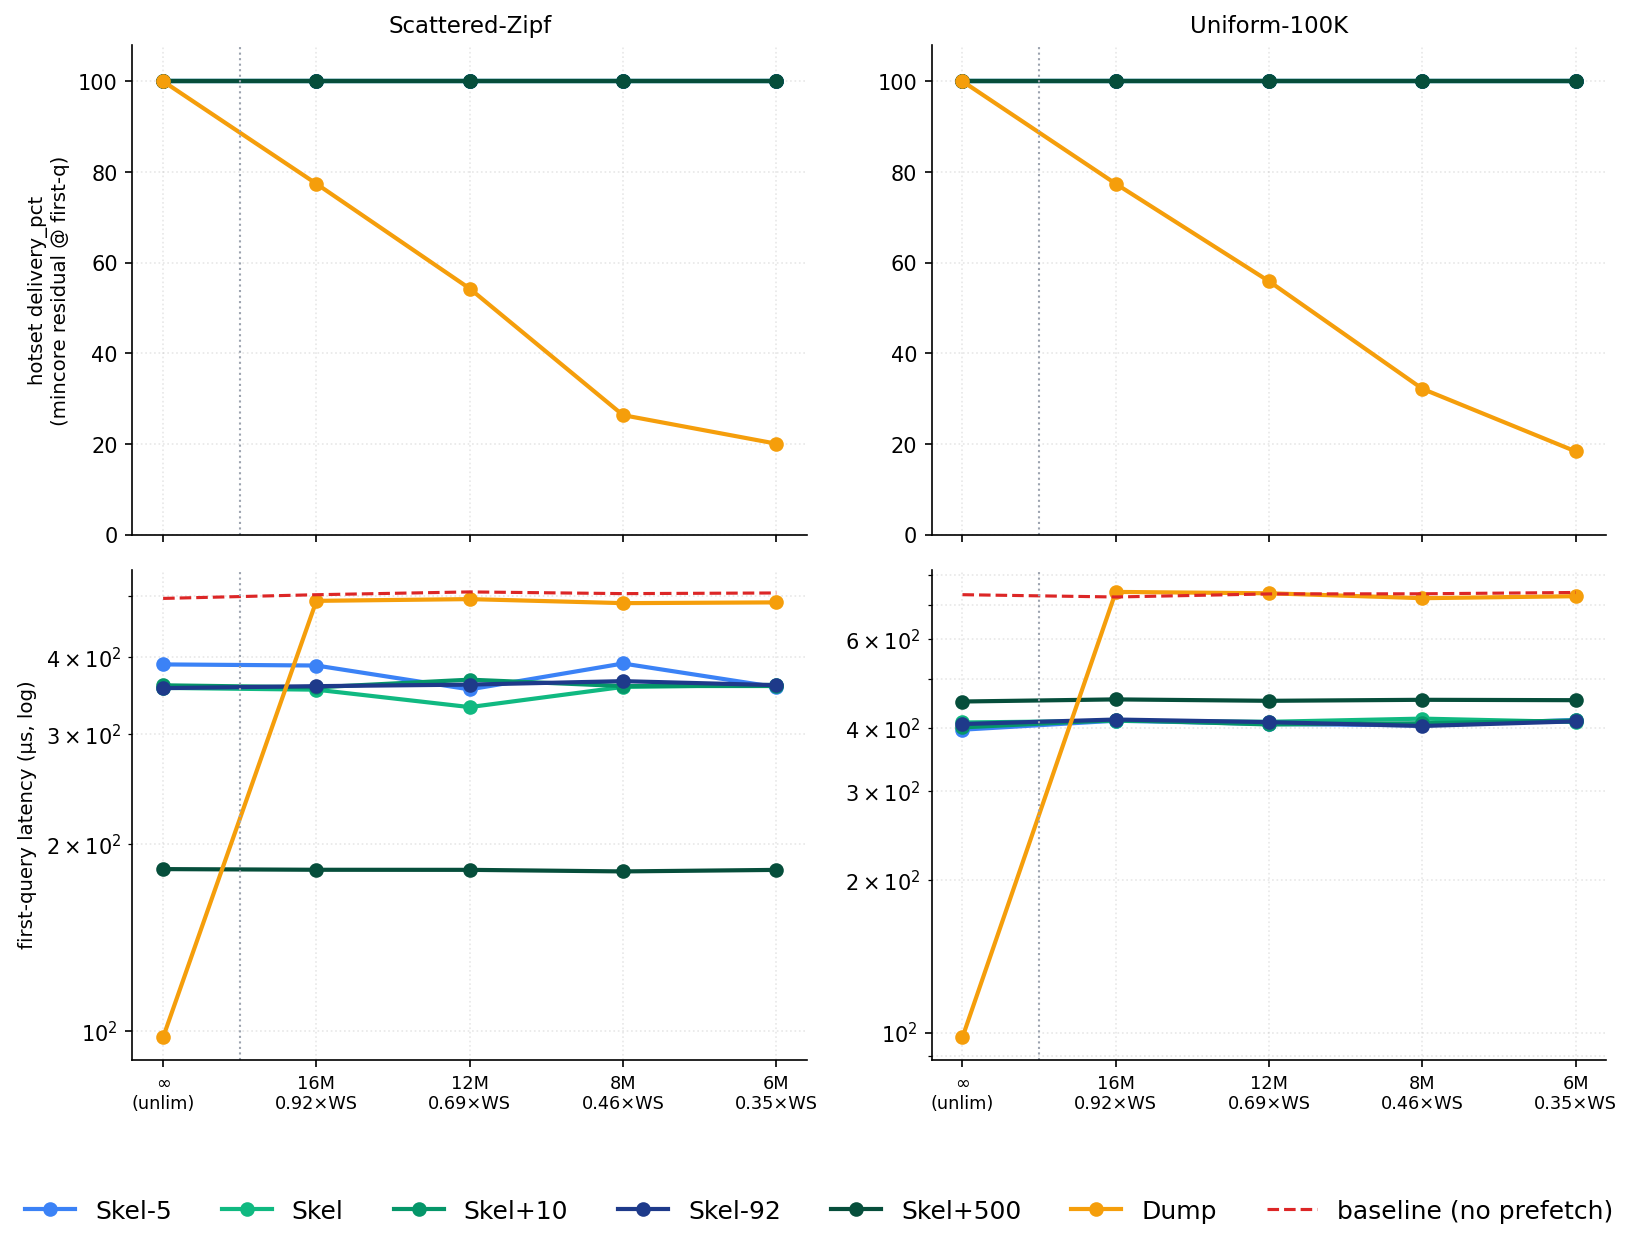
\includegraphics[width=1\linewidth]{figures/16_ram_pressure_sweep.png}
\caption{Delivery rate (top) and first-query latency (bottom) under cgroup \texttt{MemoryMax} caps. Targeted strategies keep $100\%$ delivery and flat latency, whereas Dump loses delivery linearly and collapses to baseline once delivery falls below $100\%$.}
\label{fig:ram}
\end{figure}

\subsection{First-Query Effectiveness Portability}\label{sec:eval-portability}

This experiment asks a narrower question than the workstation axes: does the first-query effectiveness of the prefetched sets survive a FaaS runtime on a different host? It does not re-evaluate end-to-end ordering. We replicate the strategy matrix on the OpenWhisk deployment of Section~\ref{sec:setup-openwhisk} and compare cells by the relative first-query reduction $R$ defined there. A cell is effective if $R \geq 0.10$, harmful if $R \leq -0.10$, and neutral otherwise, and a workstation cell is strongly effective if $R_\text{ws} \geq 0.30$. Seven of the 55 first-query cells were re-measured with position-balanced replications after low sample counts or pair-position imbalance, under a precedence rule fixed before the reruns, and every statistic below uses the revised values for those seven and the original values for the other 48.

All 41 strongly effective workstation cells remain effective on OpenWhisk (Figure~\ref{fig:portability}). Per-cell ranks correlate at Spearman $\rho$ of 0.76 over all 55 cells, 0.79 over the 46 high-confidence cells (dropping low-sample cells), and 0.81 over the 42 clean cells (also dropping four position-sensitive cells whose baseline-first and target-first subsets disagree in sign). Direction agrees in 46 of 55 cells, and the median absolute gap is $|\Delta R| \approx 0.11$
. Table~\ref{tab:portability} breaks this down by workload. Rank agreement is high on the three native traces and on Tail-Mixed ($\rho$ of 0.70 to 0.87), and Tail-Hit's low $\rho$ of 0.25 reflects a saturated control in which every cell is effective on both platforms with little rank spread, not a portability failure. High rank agreement can coexist with lower direction agreement when cells sit near a threshold, as on Uniform-600K ($\rho$ of 0.87 but 7 of 10 direction agreement, with three near-boundary cells crossing).

The nine cells that change classification all sit at the neutral margin or are low-sample or position-sensitive. The only cell harmful on OpenWhisk, \texttt{Skel-5} on Hotspot-1\%-scattered ($R_{\text{ws}} \approx +0.03$ to $R_{\text{ow}} \approx -0.60$), is workstation-neutral to begin with. The four position-sensitive cells are reported as descriptive balanced-batch estimates that reflect pair position and short-lived execution-storage state rather than a clean per-cell effect. Within the scope stated in Section~\ref{sec:contribution}, the mechanism is deployable and its first-query effectiveness is broadly consistent across the two platforms.

\begin{table}[htbp]
\centering
\caption{Per-workload first-query effectiveness portability, workstation versus OpenWhisk. Spearman $\rho$ measures rank agreement in $R$, and direction agreement counts cells whose effective / neutral / harmful class (thresholds at $\pm0.10$) matches on both platforms. The three native traces are defined in Section~\ref{sec:workloads}.}
\begin{tabular}{lccc}
\toprule
\textbf{Workload} & \textbf{Cells} & \textbf{Spearman $\rho$} & \textbf{Direction agree} \\
\midrule
Scattered-Zipf-600K   & 10 & 0.77 & 9/10  \\
Uniform-600K          & 10 & 0.87 & 7/10  \\
Hotspot-1\%-scattered & 10 & 0.82 & 8/10  \\
Tail-Mixed            & 14 & 0.70 & 11/14 \\
Tail-Hit              & 11 & 0.25 & 11/11 \\
\midrule
\textbf{All}          & 55 & 0.76 & 46/55 \\
\bottomrule
\end{tabular}
\label{tab:portability}
\end{table}

\begin{figure*}[htbp]
\centering
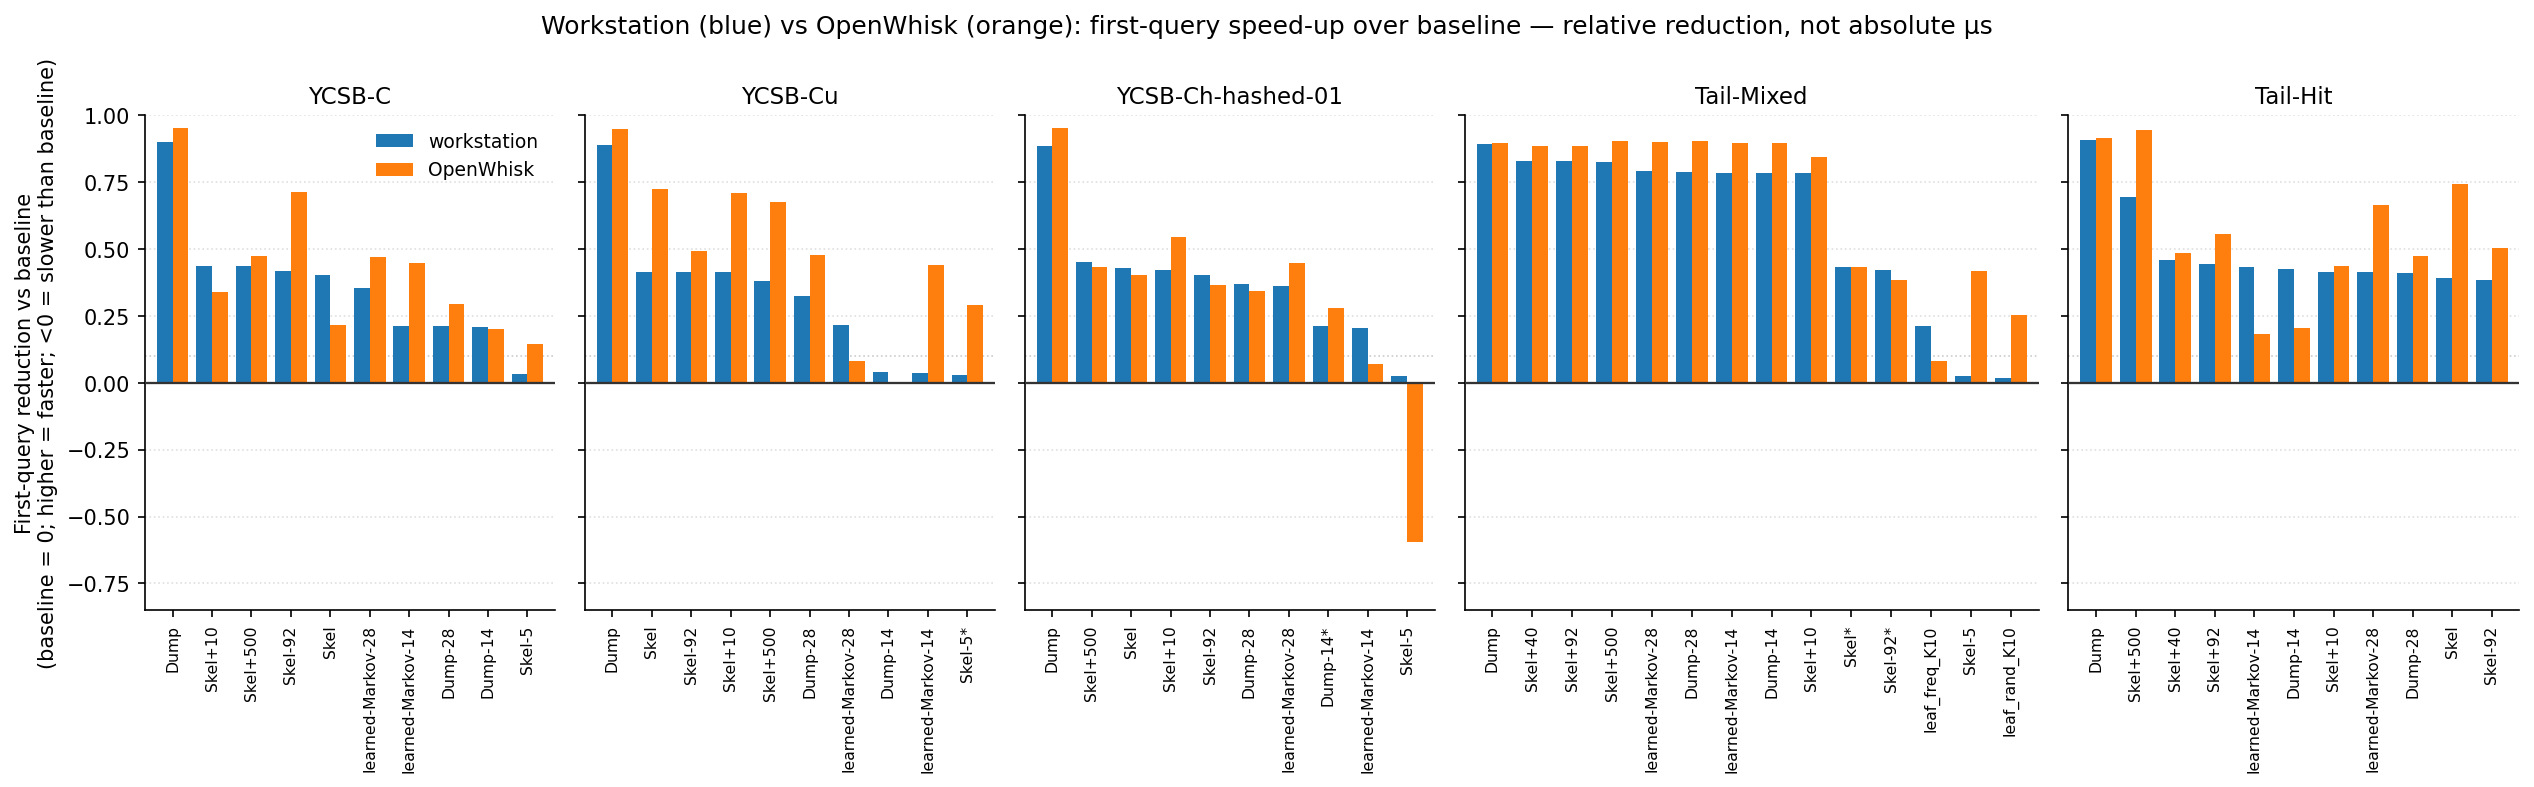
\includegraphics[width=\textwidth]{figures/19_openwhisk_effectiveness_bars.png}
\caption{Per-cell first-query effectiveness $R$ on the workstation and on OpenWhisk. All 41 strongly effective workstation cells remain effective, and disagreements cluster at the neutral margin.}
\label{fig:portability}
\end{figure*}

\subsection{Practical Guidance}\label{sec:eval-guidance}

Three rules summarize the results. First, for warm-process deployments the default is \texttt{Skel} on the Default layout: it improves end-to-end latency on every workload, survives cross-seed validation, and needs under 2 MB. Second, a small leaf budget (\texttt{Skel+10}) is worth adding only after an independently verified, stable skew, and when the read hotspot moves the durable choice is structural coverage or a periodic plan refresh rather than a frozen frequency plan. Third, \texttt{Dump} belongs to batch or average-latency settings, not the cold-start critical path: its delivery cost dominates except for the smallest working sets, and even that exception erodes as the database grows (Section~\ref{sec:eval-robustness}). \texttt{Skel-5} should not be used alone, since its single-workload wins do not survive cross-seed validation. Where only structural selection is available, prefetch the full interior set (\texttt{Skel-92}, 368 KB), which does not depend on offset order.

%\begin{table*}[htbp]
%\centering
%\begin{tabular}{p{0.16\textwidth} p{0.24\textwidth} p{0.18\textwidth} p{0.30\textwidth}}
%\toprule
%\textbf{Scenario} & \textbf{Recommended strategy} & \textbf{First-query} & \textbf{End-to-end (warm)} \\
%\midrule
%\textbf{Default} (any tail/uniform read) & \texttt{Default} original layout + \texttt{Skel} interior skeleton & $-38\%$ to $-44\%$ & $\approx$$-25\%$ to $-30\%$ robust (interior skeleton) \\
%Independently verified stable skew & add a small top-$K$ leaf budget (\texttt{Skel+10}) & up to $-64\%$ (Scattered-Zipf-100K) & Scattered-Zipf-100K $-25\%$ (\texttt{Skel}) $\to$ $-36\%$ (\texttt{Skel+10}) robust \\
%Mixed / existence-check (many not-found) & \texttt{Skel+10} & $-83\%$ (Tail-Mixed, single) & up to $\approx$$-70\%$ only when the first query is a not-found probe. Cross-seed $-55\%$ bimodal (scoped, not general) \\
%Moving hotspot / read-latest & structural coverage or periodic plan refresh & n/a & static frequency plan decays, structural coverage stable \\
%Batch / average-latency sensitive & \texttt{Dump} (cache dump) & $-80\%$ to $-91\%$ & Regresses on Scattered-Zipf-100K/Uniform-100K. On Tail-Mixed, $-16\%$ (warm, single) \\
%Multi-process shared DB & Shared cache (\texttt{MAP\_SHARED}) + background warmer, cadence $\le$ query gap & Cost fixed, benefit scales with process count & 1 second cadence maintains $\sim$26 \textmu s \\
%\bottomrule
%\end{tabular}
%\caption{Recommended strategy by deployment scenario. End-to-end values are single-instantiation warm-process results unless marked cross-seed.}
%\label{tab:guidance}
%\end{table*}

\section{Discussion and Limitations}\label{sec:discussion}

The end-to-end results come from one commodity x86 machine with a consumer NVMe SSD and one Linux kernel, so absolute microseconds are specific to that platform, and the cost-accounting methodology is what we expect to transfer to any deployment in the warm-container, cold-data state. The OpenWhisk deployment tests deployability and first-query effectiveness on a second host and runtime, within the scope stated in Section~\ref{sec:contribution}, and does not extend to other hardware classes or commercial FaaS providers. Our measurements also cover only the local-storage tier that object-storage-backed deployments interpose as a cache. The purely remote tier replaces page-cache faults with VFS-level range requests, which preserves the dependent fault chain but changes the per-fault cost by orders of magnitude, and we leave it to future work.

Absolute latencies drift by roughly $10\%$ to $15\%$ between sessions, and individual cells can shift more across machine-state groups. Diagnostics associate the drift with SSD internal state and CPU thermal conditions. Because \texttt{Dump}'s first-query latency is independent of the key distribution, we use it to monitor drift and anchor every effect to a same-batch baseline (Section~\ref{sec:stats}).

Workload coverage spans three distribution families with 10-seed sampling for within-family variation. It does not include real mixed read-write traces or other families. Tail-Mixed's robustness under memory pressure is deductive, because its 1.8 MB working set is below the measurable cgroup floor, and a larger-working-set variant is future work.

The methodology stops at the OS page cache and does not control SSD-internal FTL behavior, garbage collection, or wear leveling, and layout evolution beyond the 50,000-mutation window is unobserved. A FEMU-based study is a natural extension. Finally, the warm-process model differs from a full cold reboot by an estimated 1 to 3 \textmu s of CPU cache warm-up, below $1\%$ of the cold baseline, and a strict cold-start mode that quantifies this precisely is future work.

\section{Conclusion}\label{sec:conclusion}

Serverless functions backed by SQLite pay a cold-start penalty whenever the OS page cache is evicted between invocations, and prefetching is the natural remedy. Our argument is methodological: judging a prefetch strategy by post-prefetch first-query latency alone is insufficient, because the prefetch itself sits on the user-visible critical path. Charging it, as a cold-open and a per-page delivery term under two deployment boundaries, changes the ranking. The full cache dump that minimizes first-query latency regresses end-to-end cold starts by roughly an order of magnitude on broad workloads, because its 0.8 to 7 ms delivery cost dominates. The strategy that survives is frugal coverage: a set under 2 MB covering the B+tree interior navigation path yields a robust $25\%$ to $30\%$ warm-process end-to-end reduction across pure-hit workloads, hot leaves add a bonus only under an independently verified hotspot, and at matched footprint a frequency-ranked dump is statistically indistinguishable from the type-aware selector. Page-type knowledge therefore serves as an interpretable coverage guarantee that stays stable when the read hotspot moves, rather than as a faster selector. Physical page reordering and the small offset-ordered heuristic are negative results. No single strategy is universally optimal: the right choice depends on the deployment model and the workload's hotspot structure, with interior coverage on the default layout as the robust default. The framework is non-intrusive, uses only standard OS interfaces, and its first-query effectiveness carries over to a separate-host OpenWhisk deployment within the scope of Section~\ref{sec:contribution}. To our knowledge, this is the first work to quantify the first-query versus end-to-end trade-off for SQLite cold starts at syscall granularity.

Three directions follow. Page-type knowledge can be pushed below the file abstraction, where NVMe stream directives or ZNS could segregate interior and leaf pages without the leaf-displacement penalty of file-level reordering and shield the layout from garbage collection. In the object-storage regime the same skeleton-first selection becomes a VFS question of which pages to coalesce into one range request, and the trade-offs we quantify grow with millisecond per-fault costs. A continuous prefetch that maintains residency across invocations would extend the framework to steady state, but it moves the design point into the high-frequency, kernel-level regime of vmcache~\cite{Leis2023} and would require re-evaluating the deployment model. More broadly, we argue that cost accounting, not first-query latency alone, should be the evaluation standard for cold-start prefetching.

%\clearpage

\bibliographystyle{ACM-Reference-Format}
\bibliography{sample}

\end{document}
\endinput
